% !TeX root = ../thesis.tex

\begin{savequote}[75mm]
    The most exciting phrase to hear in science, the one that heralds new discoveries, is not 'Eureka!' but 'That's funny...'
    \qauthor{Isaac Asimov}
    \end{savequote}

\chapter{Assess Health Data Science Methods With Limited Data Access}\label{chap:goal2}
\initial{T}his chapter delves into the assessment of health data science methods under the constraints of limited data access, as outlined in sections \ref{subsec:distributed} and \ref{subsec:benchmark}. It emphasizes the importance of developing and evaluating data science techniques that can operate effectively even when direct access to comprehensive datasets is restricted. In section \ref{subsec:distributed}, the focus is on distributed data approaches, which allow for the analysis of health data across multiple locations without the need to centralize the information. This method is crucial for maintaining privacy and security, especially in sensitive health data contexts. Meanwhile, section \ref{subsec:benchmark} discusses benchmarking strategies for these methodologies, providing a framework to evaluate their effectiveness and reliability. These benchmarks are essential to ensure that the methods yield accurate and useful insights, despite the limitations in data accessibility.


\section{Leveraging Distributed Systems in Healthcare: is it Advisable?}\label{subsec:distributed}
This section is based on the paper entitled "Evaluating distributed-learning algorithms on real-world healthcare data" \cite{coutinho-almeidaEvaluatingDistributedlearningRealworld2024}. This paper was focused on the fact that access to healthcare data is often laboursome and time-consuming. So we evaluated the distributed paradigm to its gold-standard, the centralised paradigm. We used 9 real-world datasets of obstetrics \acp{ehr} and compared the performance of several \ac{ml} algorithms in both paradigms. We concluded that the distributed paradigm is a valid alternative to the centralised paradigm, with the added benefit of not requiring heavy data sharing.

\subsection{Introduction}
% !TeX root = ../../thesis.tex

%As the use of \ac{ai} is increasing in the healthcare space \cite{deep_learning_increase_health}, increased demand for ethical usage of personal patient data is occurring as well \cite{ehtical_use_ml}. This has been happening both on the governmental side, with several regulations passed to protect citizens' data and personal information (such as \ac{gdpr} in the \ac{eu} \cite{gdpr_article} and \ac{hipaa} in the \ac{us} \cite{hippa}), and on the public side, with an increased concern with continuous data breaches across institutions \cite{abdulrahmanSurveyFederatedLearning2021}. So,  we are now faced with a dilemma on a compromise between what is possible to do with the available data and what should be done regarding patient privacy \cite{swarm_learning}. This is the main reason why health institutions implement burdensome processes and methodologies for sharing patient data, often costing a great deal of time, money, and human resources, seldomly overtaking the ideal time frame for analysing such data.
%Due to these privacy concerns, the traditional method for using data in healthcare is, nowadays, by focusing on data from a single institution in order to predict or infer something regarding those patients; this could be understood as local learning. This approach has some drawbacks, namely data quantity, data quality and possible class imbalance \cite{rajkomarMachineLearningMedicine2019}, never quite raising into its full potential for promoting best healthcare practices
%\cite{federated_healthcare_informatics,usage_ai_healthcare,wangAIHealthState2019} with data sharing between institutions.
%In order to overcome this issue, there are a few, more complex, systems that aggregate data from several institutions, so more robust algorithms could be trained. However, this globally centralised aggregation of data encompasses a very important data breach hazard. 

%This is the setting where distributed learning could create a greater impact. A halfway point between local and centralised learning is where we train several models, one in each institution (or silo), and where the sole information that leaves the premises is a trained model or its metadata. A distributed model is built as the aggregation of all the local models, consequently aiming to create a model similar to one globally trained with all the data in a centralised server. However, the distributed model never contacted with any data, only the local models did. This provides the opportunity to create better models, improve data protection, reduce training time and cost and provide better scaling capabilities  \cite{jatainContemplativePerspectiveFederated2021}.

%including federated-learning approaches, where a central system orchestrates the operation \cite{federated_learning_intro} or a swarm/peer-to-peer framework where silos communicate with each other. However,
%There are already some implementations of distributed systems in the healthcare space, but we lack a robust understanding of how these models behave with real data, when compared with the classical models built with all the aggregated data. Additionally, the main issues regarding the development and implementation of such systems in healthcare are still elusive.
%So we aim to understand how distributed mechanisms behave compared to using all data in the healthcare space and if they are a suitable replacement for traditional machine-learning pipelines. The contributions of this paper are:
%\begin{myitemize}
%    \item Understand how to address the lack of data quality of real-world data regarding distributed model creation;
%    \item Evaluate a distributed model against its local counterparts;
%    \item Measure the prediction performance difference between a distributed model and a centralised one;
%    \item Identify the capabilities of a distributed model to track population changes on the local datasets;
%    \item Open a research path for using distributed models to predict several target variables in obstetrics clinical research.
%\end{myitemize}


As the use of \ac{ai} is increasing in the healthcare space \cite{deep_learning_increase_health}, increased demand for ethical usage of personal patient data is occurring as well \cite{ehtical_use_ml}. This has been happening both on the governmental side, with several regulations passed to protect citizens' data and personal information (such as \ac{gdpr} in the \ac{eu} \cite{gdpr_article} and \ac{hipaa} in the \ac{us} \cite{hippa}), and on the public side, with an increased concern with continuous data breaches across institutions \cite{abdulrahmanSurveyFederatedLearning2021}. So,  we are now faced with a dilemma on a compromise between what is possible to do with the available data and what should be done regarding patient privacy \cite{swarm_learning}. This is the main reason why health institutions implement burdensome processes and methodologies for sharing patient data, often costing a great deal of time, money, and human resources, seldomly overtaking the ideal time frame for analysing such data.
Due to these privacy concerns, the traditional method for using data in healthcare is, nowadays, by focusing on data from a single institution in order to predict or infer something regarding those patients; this could be understood as local learning. This approach has some drawbacks, namely data quantity, data quality and possible class imbalance \cite{rajkomarMachineLearningMedicine2019}, never quite raising into its full potential for promoting the best healthcare practices
\cite{federated_healthcare_informatics,usage_ai_healthcare,wangAIHealthState2019} with data sharing between institutions.
In order to overcome this issue, there are a few, more complex, systems that consolidate data from several institutions, so more robust algorithms could be trained. However, this globally centralised consolidation of data encompasses a very important data breach hazard. 

This is the setting where distributed learning could create a greater impact. A halfway point between local and centralised learning is where we train several models, one in each institution (or silo), and where the sole information that leaves the premises is a trained model or its metadata. A distributed model is built as the aggregation of all the local models, consequently aiming to create a model similar to one globally trained with all the data in a centralised server. However, the distributed model never contacted with any data, only the local models did. This provides the opportunity to create better models, improve data protection, reduce training time and cost and provide better scaling capabilities  \cite{jatainContemplativePerspectiveFederated2021}.

%including federated-learning approaches, where a central system orchestrates the operation \cite{federated_learning_intro} or a swarm/peer-to-peer framework where silos communicate with each other. However,
%There are already some implementations of distributed systems in the healthcare space, but we lack a robust understanding of how these models behave with real data, when compared with the classical models built with all the aggregated data. So we aim to understand how distributed mechanisms behave compared to using all data in the healthcare space and if they are a suitable replacement for traditional machine-learning pipelines. The contributions of this paper are:

While numerous multi-institutional initiatives have successfully established integrated data repositories for healthcare research, there remains an incomplete understanding of the performance and scalability of distributed systems when directly compared to traditional, centralised models. Specifically, the nuanced behaviours of these distributed frameworks under real-world data conditions—contrasted against classical models that utilize consolidated data—have yet to be fully delineated. This paper aims to critically evaluate the efficacy and suitability of distributed mechanisms within the healthcare domain, assessing their potential as viable alternatives to conventional machine-learning pipelines. The contributions of this paper include:

\begin{myitemize}
    \item Evaluate a distributed model against its local counterparts;
    \item Measure the prediction performance difference between a distributed model and a centralised one;
%    \item Identify the capabilities of a distributed model to track population changes on the local datasets;
    %\item Understand how to address the lack of data quality of real-world data regarding distributed model creation;

  %  \item Open a research path for using distributed models to predict several target variables in obstetrics clinical research.
\end{myitemize}

\subsection{Theoretical background and Related Work}
Distributed learning \cite{distributed} can be understood as training several models in a different setting and then aggregating them as a whole. There are two main branches of these approaches, distinguishable by the existence of a central orchestrator server: federated learning where such an entity exists, and peer-to-peer (or swarm) \cite{swarm_learning} learning where it does not. 
Even though distributed learning has been receiving a lot of attention recently, only some of its concepts have been focused on, mainly distributed-deep learning with a federated learning approach \cite{xuFederatedLearningHealthcare2021,leeFederatedLearningClinical2020}. These methods use the strength of neural networks and several algorithms like federated averaging to create distributed models capable of handling complex data like text, sound, or image \cite{prayitnoSystematicReviewFederated2021}. However, considering that there are great amounts of information, especially in healthcare, stored as tabular data \cite{alvarezsanchezTAQIHToolTabular2019,dimartinoExplainableAIClinical2022,payrovnaziriExplainableArtificialIntelligence2020} and that neural networks are often not the best tool for such data structures \cite{borisovDeepNeuralNetworks2022a}, there is a lack of knowledge in the traditional machine learning techniques in a distributed manner.
%Federated Learning was introduced in 2016 \cite{konecny_federated_2016,mcmahanFederatedLearningDeep2016} and it was called federated since "the learning task is solved by a loose federation of participating devices (which we refer to as clients) which are coordinated by a central server" \cite{konecny_federated_2016}. Federated learning has two main architectures: a) horizontal and b) vertical  \cite{yangFederatedMachineLearning2019b}. 
%Horizontal refers to having the same features in all silos, but different populations in each silo. Vertical refers to having different features across silos for the same population. Then we have other approaches that expand the concept of federated learning with previous machine learning and deep learning methodologies such as transfer learning, reinforcement learning \cite{liuSystematicLiteratureReview2020} and quantum machine-learning \cite{quantum-fed-ml}. 
%Federated learning can also be classified by the information flow. Model data can be shared only with the main central server, as in more traditional methods, but also being incremental, sharing data model sequentially between silos, with central server orchestration \cite{cyclic_distribution}. 

Nevertheless, there have been some health-related  distributed machine-learning projects successfully implemented, such as euroCAT  \cite{eurocat} which implemented an infrastructure across five clinics in three countries. \ac{svm} models were used to learn from the data distributed across the five clinics. Each clinic has a connector to the outside where only the model's parameters are passed to the central server which acts as a master deployer regarding the model training with the radiation oncology data.
Also, ukCAT \cite{ukcat} did similar work, with an added centralised database in the middle, but the training being done with a decentralized system.
%Other methods and approaches have been also evaluated such as the work of Brisimi et. al. \cite{brisimi_federated_2018}  for predicting hospitalisations or deep learning methods oriented to analysing medical imaging \cite{chang_distributed_2018}, evaluating histological samples \cite{pathology-fl} and finally, some preprints showing the impact of federated learning regarding COVID-19 prediction \cite{vaid_federated_2020}. For a sound review please redirect to Zerka et al. \cite{zerkaSystematicReviewPrivacyPreserving2020a}

Finally, a few works have explored the evaluation of models in a distributed manner, for example, comparing  centralised machine learning, distributed machine learning and federated learning on MNIST dataset \cite{performance_evaluation_1}. Also, works that evaluate federated learning on MNIST, MIMIC-III and PhysioNet ECG datasets, but not in comparison with other methods  \cite{performance_evaluation_2}. The work by Tuladhar and colleagues \cite{distributed} uses healthcare images and/or public and curated datasets.
As far as we know, this is the first time a distributed machine learning evaluation is done with real-world clinical data from several different data sources.
\subsection{Materials}
Clinical data was gathered from nine different Portuguese hospitals regarding obstetric information, pertaining to admissions from 2019 to 2020. This originated nine different files representing different sets of patients but with the same features associated to them. The software for collecting data was the same in every institution (although different versions existed across hospitals) - ObsCare. The data columns are the same in every hospital's database. Each hospital was considered a silo and summary statistics of the different silos are reported in the tables \ref{tab:distributed_materials_1} and \ref{tab:distributed_materials_2}. The data dictionary is in appendix \ref{appendix:data_dict}.
%TC:ignore

{\small
\begin{table}[!ht]

\caption[Silos overview.]{\label{tab:distributed_materials_1}Silos overview. categorical columns have a snippet of the most used category and a percentage. Continuous variables have a mean and standard deviation. Abbreviation meaning in the appendix. The last row is the number of patients. * columns were used as target.}

\centering
% !TeX root = ../../thesis.tex
\newcolumntype{L}{>{\scriptsize}l}  % "small" can be changed to "scriptsize" or "footnotesize" for even smaller text

\begin{tabular}{LLLLLLL}
   \toprule
      Variable &               Silo 1 &               Silo 2 &               Silo 3 &               Silo 4 &               Silo 5 &                Total \\
   \midrule
   \hspace*{2mm} N (total) &              8039 &                 8566 &                 4989 &                 2364 &                18177 &                80874 \\
   
   \textbf{Actual Type of Delivery C (\%)}& 10 (52.6) & 3 (51.6) & 3 (57.8) & 3 (61.8) & 9 (61.5) & 11 (52.9) \\
   
   Bishop Score C (\%)&  15 (98.5) & 15 (78.8) & 13 (97.4) & 16 (86.4) & 15 (97.4) & 16 (95.3) \\
   
   \textbf{Blood Group C (\%)}& 9 (39.9) & 10 (39.9) & 9 (39.3) & 11 (37.9) & 10 (40.9) & 14 (40.5) \\
   
   \textbf{Body Mass Index $\mu (\sigma)$ } & 25.2 (8.6) & 25.2 (6.2) & 25.0 (5.3) & 25.0 (8.9) & 24.9 (7.8) & 25.1 (7.0) \\
   
   Cervical Consistency C (\%) & 4 (98.6) & 4 (83.4) & 4 (99.3) & 4 (87.4) & 4 (97.5) & 4 (96.5) \\
   
   Cervical Position C (\%)&  4 (98.6) & 4 (83.3) & 4 (99.3) & 4 (87.5) & 4 (97.6) & 4 (96.6) \\
   
   \textbf{Delivery Type C (\%)}& 6 (43.4) & 6 (53.5) & 5 (44.4) & 7 (52.2) & 7 (49.3) & 8 (51.3) \\
   
   Dilatation C (\%)&5 (98.5) & 5 (83.1) & 5 (99.3) & 5 (87.2) & 5 (97.5) & 5 (96.5) \\
   
   Effacement C (\%)& 5 (98.6) & 5 (83.2) & 5 (99.3) & 5 (87.2) & 5 (97.5) & 5 (96.5) \\
   
   Fetal Station  C (\%)&  5 (98.6) & 5 (83.3) & 5 (99.3) & 5 (87.9) & 5 (97.5) & 5 (96.6) \\
   
   \textbf{Followed physician C (\%)} & 3 (99.2) & 4 (92.2) & 3 (99.1) & 3 (94.3) & 3 (99.0) & 4 (97.9) \\
   
   \textbf{\begin{minipage}{3.8cm}\setstretch{0.65}Followed physician hospital delivery C (\%)\vspace{1mm}\end{minipage}}&  2 (87.6) & 2 (75.8) & 2 (81.4) & 2 (52.2) & 2 (71.0) & 2 (69.0) \\
   
   \textbf{\begin{minipage}{3.8cm}\setstretch{0.65}Followed physician primary care C (\%)\vspace{1mm}\end{minipage}}&  2 (61.3) & 2 (52.8) & 2 (78.1) & 2 (50.4) & 2 (70.4) & 2 (67.6) \\
   
   \begin{minipage}{3.8cm}\setstretch{0.65}Followed physician private clinic C (\%)\vspace{1mm}\end{minipage}&  2 (81.8) & 2 (85.0) & 2 (80.6) & 2 (78.8) & 2 (73.3) & 2 (75.8) \\
   
   Gestational Diabetes C (\%)&2 (87.7) & 2 (90.0) & 2 (90.2) & 2 (90.8) & 2 (89.8) & 2 (89.5) \\
   
   
   Induced Delivery  C (\%)& 2 (97.8) & 2 (83.9) & 2 (93.3) & 2 (91.9) & 2 (98.5) & 2 (92.5) \\
   
   \textbf{Mother Age $\mu (\sigma)$ } & 31.1 (5.7) & 30.7 (5.6) & 31.1 (5.9) & 31.1 (6.3) & 31.3 (5.6) & 31.1 (5.6) \\
   
   
   \begin{minipage}{3.9cm}\setstretch{0.65}Nr Deliveries forceps C (\%)\end{minipage} & 4 (99.2) & 3 (83.3) & 4 (94.3) & 4 (95.8) & 3 (60.1) & 5 (82.6) \\
   
   
   \begin{minipage}{3.9cm}\setstretch{0.65}Nr Deliveries no assistance C (\%)\vspace{1mm}\end{minipage} & 10 (74.7) & 9 (60.3) & 9 (74.9) & 9 (67.3) & 11 (45.4) & 12 (60.3) \\
   
   \begin{minipage}{3.9cm}\setstretch{0.65}Nr Deliveries vacuum C (\%)\vspace{1mm}\end{minipage} &  5 (90.4) & 4 (79.9) & 4 (89.0) & 4 (93.1) & 5 (55.3) & 5 (77.4) \\
   
   Nr of C-sections C (\%) & 6 (87.9) & 6 (72.6) & 5 (86.1) & 5 (89.5) & 6 (62.1) & 6 (74.6) \\
   
   \textbf{Nr of Pregnancies C (\%)} &  11 (40.9) & 11 (43.1) & 13 (39.1) & 12 (38.7) & 16 (42.8) & 19 (42.1) \\
   
   \textbf{Nr of born babies C (\%)} & 10 (44.8) & 10 (41.4) & 10 (36.9) & 10 (42.0) & 12 (35.3) & 12 (38.8) \\
   
   \textbf{Nr of consultations $\mu (\sigma)$ } &  7.3 (4.7) & 7.0 (6.4) & 6.4 (3.9) & 5.5 (3.6) & 10.5 (5.1) & 8.4 (5.1) \\
   
   Pelvis Adequacy C (\%) &4 (95.4) & 4 (77.7) & 4 (90.1) & 3 (96.9) & 4 (81.2) & 4 (82.6) \\
   
   \textbf{Position Admission C (\%)}  &  5 (88.5) & 6 (78.0) & 6 (51.8) & 3 (95.9) & 6 (71.3) & 7 (73.1) \\
   
   
   \textbf{Position on Delivery C (\%)} &5 (91.5) & 5 (94.4) & 5 (94.7) & 5 (95.5) & 5 (94.3) & 5 (93.9) \\
   
   \textbf{Pregnancy Type C (\%)} &  7 (62.1) & 7 (90.5) & 7 (85.4) & 7 (63.0) & 7 (89.2) & 7 (85.4) \\
   
   \textbf{Robson Group C (\%)} & 11 (22.4) & 11 (20.1) & 10 (23.8) & 10 (80.5) & 11 (27.7) & 11 (24.4) \\
   
   \begin{minipage}{3.7cm}\setstretch{0.65}Rupture amniotic pocket before delivery C (\%)\end{minipage} &  2 (91.1) & 2 (93.6) & 2 (89.3) & 2 (91.6) & 2 (84.6) & 2 (88.5) \\
   
   Smoker C (\%) & 2 (84.4) & 2 (85.2) & 2 (87.2) & 2 (89.7) & 2 (87.9) & 2 (88.1) \\
   
   \textbf{Spontaneous Delivery C (\%)} &  2 (70.3) & 2 (74.7) & 2 (64.8) & 2 (64.3) & 2 (59.7) & 2 (64.9) \\
   
   \textbf{Weeks on Admission C (\%)} &    38.1 (3.5) &    38.8 (2.2) &    38.9 (1.6) &    38.8 (2.4) &    38.6 (2.1) &    38.7 (2.2) \\
   
   
   \textbf{Weeks on Delivery $\mu (\sigma)$ } &    38.5 (2.8) &    38.9 (2.0) &    39.1 (1.7) &    39.0 (2.3) &    38.9 (2.0) &    38.9 (2.0) \\
   
   Weight on Admission $\mu (\sigma)$  &   81.4 (14.9) &   79.5 (14.5) &   78.0 (15.2) &   79.6 (16.3) &   78.3 (14.2) &   78.8 (14.5) \\
   
   
   \textbf{\begin{minipage}{3.3cm}\setstretch{0.65}Weight start  of pregnancy $\mu (\sigma)$ \vspace{1mm}\end{minipage}} &   66.4 (14.4) &   66.1 (13.5) &   65.5 (14.1) &   65.5 (14.1) &   65.5 (14.4) &   66.0 (14.1) \\
   \bottomrule
   \end{tabular}
   
   
\end{table}
}
\newpage

{\small
\begin{table}[!ht]

\caption[Silos overview part 2.]{\label{tab:distributed_materials_2}Silos overview part 2. categorical columns have a snippet of the most used category and a percentage. Continuous variables have a mean and standard deviation. Abbreviation meaning in the appendix. The last row is the number of patients. * columns were used as target.}
\centering
% !TeX root = ../../thesis.tex

\begin{tabular}{llllll}
   \toprule
   Variable &               Silo 6 &               Silo 7 &               Silo 8 &               Silo 9 &                Agrr. \\
   \midrule
   
   \hspace*{2mm}  N (total) &                12002 &                 8258 &                 6693 &                11786 &                80874 \\
   
   \textbf{Actual Type of Delivery C (\%)} & 10 (63.8) & 0 (100) & 10 (50.1) & 9 (64.6) & 11 (52.9) \\
   Bishop Score C (\%) & 14 (99.3) & 15 (97.9) & 14 (99.2) & 15 (95.0) & 16 (95.3) \\
   \textbf{Blood Group C (\%)} & 13 (41.6) & 10 (39.2) & 10 (40.1) & 10 (41.7) & 14 (40.4) \\
   \textbf{Body Mass Index $\mu (\sigma)$ } & 24.9 (5.1) & 24.9 (7.0) & 24.8 (8.0) & 25.7 (5.6) & 25.1 (7.0) \\
   Cervical Consistency C (\%)  & 4 (99.5) & 4 (99.7) & 4 (99.5) & 4 (96.9) & 4 (96.5) \\
   Cervical Position C (\%) & 4 (99.5) & 4 (99.7) & 4 (99.5) & 4 (96.9) & 4 (96.5) \\
   \textbf{Delivery Type C (\%)} & 6 (54.3) & 5 (52.1) & 5 (47.8) & 5 (59.0) & 8 (51.3) \\
   Dilatation C (\%) & 5 (99.5) & 5 (99.7) & 5 (99.5) & 5 (96.9) & 5 (96.5) \\
   Effacement C (\%)  & 5 (99.5) & 5 (99.7) & 5 (99.5) & 5 (96.9) & 5 (96.5) \\
   Fetal Station C (\%) & 5 (99.5) & 5 (99.7) & 5 (99.5) & 5 (96.9) & 5 (96.6) \\
   \textbf{Followed physician C (\%)} & 3 (96.9) & 3 (99.4) & 3 (97.8) & 3 (99.2) & 4 (97.8) \\
   \textbf{\begin{minipage}{3.8cm}\setstretch{0.65}Followed physician hospital delivery C (\%)\vspace{1mm}\end{minipage}}& 2 (62.1) & 2 (63.2) & 2 (69.4) & 2 (83.1) & 2 (69.0) \\
   \textbf{\begin{minipage}{3.8cm}\setstretch{0.65}Followed physician primary care C (\%)\vspace{1mm}\end{minipage}} & 2 (53.1) & 2 (86.7) & 2 (63.1) & 2 (87.3) & 2 (67.6) \\
   \begin{minipage}{3.9cm}\setstretch{0.65}Followed physician private clinic C (\%)\vspace{1mm}\end{minipage} & 2 (68.2) & 2 (73.5) & 2 (71.0) & 2 (78.1) & 2 (75.8) \\
   Gestational Diabetes C (\%)  & 2 (92.2) & 2 (88.2) & 2 (89.9) & 2 (86.8) & 2 (89.5) \\
   Induced Delivery C (\%) & 2 (91.9) & 2 (85.9) & 2 (87.4) & 2 (93.9) & 2 (92.5) \\
   \textbf{Mother Age $\mu (\sigma)$ }  & 31.3 (5.2) & 31.4 (5.4) & 31.5 (5.6) & 30.1 (5.6) & 31.1 (5.6) \\
   
   \begin{minipage}{3.9cm}\setstretch{0.65}Nr Deliveries forceps C (\%)\vspace{1mm}\end{minipage} & 4 (82.0) & 4 (86.0) & 3 (94.0) & 4 (89.3) & 5 (82.6) \\
   \begin{minipage}{3.9cm}\setstretch{0.65}Nr Deliveries no assistance C (\%)\vspace{1mm}\end{minipage}  & 8 (58.8) & 9 (61.2) & 10 (68.9) & 9 (61.5) & 12 (60.3) \\
   \begin{minipage}{3.9cm}\setstretch{0.65}Nr Deliveries vacuum C (\%)\vspace{1mm}\end{minipage}& 4 (78.9) & 4 (81.6) & 4 (88.0) & 5 (82.3) & 5 (77.4) \\
   Nr of C-sections C (\%) & 6 (69.1) & 6 (74.5) & 5 (85.5) & 6 (77.8) & 6 (74.6) \\
   \textbf{Nr of Pregnancies C (\%)} & 13 (44.2) & 9 (42.9) & 11 (42.0) & 13 (40.2) & 19 (42.1) \\
   \textbf{Nr of born babies C (\%)} & 9 (38.4) & 9 (42.6) & 10 (41.2) & 10 (43.2) & 12 (38.8) \\
   \textbf{Nr of consultations $\mu (\sigma)$ } & 6.8 (4.0) & 7.7 (3.2) & 9.3 (4.5) & 8.9 (5.5) & 8.4 (5.1) \\
   Pelvis Adequacy  C (\%)  & 4 (89.6) & 4 (52.9) & 3 (93.1) & 4 (81.5) & 4 (82.6) \\
   \textbf{Position Admission C (\%)} & 6 (84.5) & 7 (61.3) & 5 (89.2) & 4 (74.2) & 7 (73.1) \\
   \textbf{Position on Delivery C (\%)} & 5 (93.0) & 5 (93.6) & 5 (94.8) & 5 (94.2) & 5 (93.9) \\
   
   \textbf{Pregnancy Type C (\%)} & 7 (88.0) & 7 (85.4) & 7 (86.0) & 7 (92.9) & 7 (85.4) \\
   \textbf{Robson Group C (\%)}& 11 (27.2) & 11 (24.7) & 11 (21.4) & 11 (26.7) & 11 (24.4) \\
   \begin{minipage}{3.7cm}\setstretch{0.65}Rupture amniotic pocket before delivery C (\%)\vspace{1mm}\end{minipage} & 2 (85.0) & 2 (84.4) & 2 (89.9) & 2 (93.8) & 2 (88.5) \\
   Smoker C (\%) & 2 (91.0) & 2 (90.7) & 2 (85.5) & 2 (89.9) & 2 (88.1) \\
   \textbf{Spontaneous Delivery C (\%)} & 2 (64.9) & 2 (64.0) & 2 (64.7) & 2 (62.9) & 2 (64.9) \\
   Weeks on Admission $\mu (\sigma)$ & 38.7 (1.8) & 39.0 (2.0) & 38.6 (2.1) & 38.8 (1.9) & 38.7 (2.2) \\
   \textbf{Weeks on Delivery $\mu (\sigma)$ }  & 38.8 (1.8) & 39.2 (1.7) & 38.7 (2.0) & 39.0 (1.6) & 38.9 (2.0) \\
   \textbf{Weeks on Admission $\mu (\sigma)$ } & 77.7 (13.4) & 79.2 (14.7) & 76.7 (13.0) & 83.1 (15.2) & 78.8 (14.5) \\
   \textbf{\begin{minipage}{3.3cm}\setstretch{0.65}Weight start of pregnancy $\mu (\sigma)$ \vspace{1mm}\end{minipage}}  & 65.6 (13.5) & 66.0 (13.7) & 65.6 (14.1) & 67.4 (14.6) & 66.0 (14.1) \\
   
   
   
   \bottomrule
   \end{tabular}
   

\end{table}
}
%TC:endignore

\subsection{Methods}
% !TeX root = ../../thesis.tex

The section will cover the steps we took for evaluating the models. We first addressed the preprocessing of the data, then the training of the models and finally the evaluation of the models. The evaluation was done by comparing the performance of the distributed model with the local and centralised models. The performance was measured by the AUROC, AUPRC, RMSE and MAE. The results were then compared using a 2-sample T-test.
\subsubsection{Preprocessing}

The initial dataset underwent preprocessing by eliminating attributes that were missing more than 90\% of their data across all storage units (or silo). We standardized the representation of missing values, which varied widely, including representations such as "-1" "missing" or simply blank spaces. For imputation, we utilized the mean for continuous variables (calculated within site) and introduced a special category (NULLIMP) for categorical variables. We converted all categories into numerical values based on a predefined mapping that covered all potential categories across the datasets. Although this approach introduces an ordinal relationship and potential bias is created among features, we disregarded this concern because the methodology was uniformly applied across all datasets intended for training local, distributed and centralised. These preprocessing tasks were executed once for each dataset and silo.

However, in the context of training classification models, it is crucial that all classes of the target variable are known at the time of training and are represented in each split of the cross-validation process. To address this, we employed SMOTE \cite{smote} to up-sampled low-frequency target classes. We established a threshold of n$<$25 for low-frequency variables to ensure that each cross-validation split contained at least two instances of the class—although a minimum of 10 instances (10 splits) might suffice, we opted for 25 to mitigate potential distribution issues and have at least two examples of the class in each split. Additionally, we created dummy rows for missing target classes by imputing the mean for continuous variables and the mode for categorical variables (calculated within site). The necessity for up-sampling and missing variable creation was evaluated and applied as needed for each training session and for each target, considering that each session's split could result in a training set lacking instances of low-frequency classes.

All procedures were coded in python 3.9.7 with the usage of the scikit-learn library \cite{scikit-learn} and mlxtend library \cite{mlxtend}.


\subsubsection{Model Training}
To avoid pitfalls of inductive bias from a certain learning strategy, we learned six different models (i) Decision Trees, (ii) Bayesian methods, (iii) a logistic regression model with Stochastic Gradient Descent, (iv) K-nearest neighbours, (v) AdaBoost and (vi) Multi-layer Perceptron. The decision was to create diversity in the models used, in order to assess if the training methodology could have an impact on distributed model creation.
The distributed model was an ensemble of models from each silo on a weighted soft-voting basis. The weights were defined by weighted averages of the scores each model obtained in the training set. Then the final result is obtained by creating a weighted average of the class predictions for classification and a weighted average for regression. A model like this can be implemented with peer-to-peer or federated approaches.
Nineteen features were used as target outcomes. These features were selected by filtering by the percentage of null values (below 50\%). This choice was related to maintaining a equilibrium between having a wide range of variables to test how the target variables affects the outcome and having target variables that did go through an harsh imputation mechanism. For categorical outcomes, thirteen were selected (AA - Position Admission; ANP - Position on Delivery; AGESTA - Nr of Pregnancies; APARA - Nr of born babies; GS - Blood Group; GR - Robson Group; TG -Pregnancy Type; TP - Delivery Type; TPEE - Spontaneous Delivery; TPNP - Actual Type of Delivery; V - Followed physician; VCS - Followed physician primary care; VNH - Followed physician hospital delivery;). For continuous variables, six were selected (IA - Mother Age; IGA - Weeks on Admission; IMC - BMI; NRCPN - Nr of consultations; PI - Weight start of pregnancy; SGP - Weeks on Delivery;). Details can be seen in tables \ref{tab:1} and \ref{tab:1.2}.
Local models were built with each silo's data. The centralised model was trained with a training dataset from all the silos combined. 


%TC:ignore
\subsubsection{Model Performance Evaluation}

All models were built for a certain outcome variable with a repeated cross-validation (2 times and 10 splits each) and then compared, over 10 stochastic runs, with evaluation being performed on a test set held out from each silo. By performing cross-validation twice, we aimed to generate a more robust estimation of the model’s performance metrics by averaging the results over two separate runs, each partitioning the data differently. This approach is particularly useful in scenarios where data is limited or highly variable, as it provides a clearer insight into the model's expected performance in unseen data scenarios. The metrics used for classification models were Weighted Area Under the Receiver Operating Characteristic Curve (AUROC) computed as One-versus-Rest, Weighted Area Under the Precision-Recall Curve (AUPRC). The metrics for regression models were Root Mean Squared Error (RMSE) and Mean Absolute Error (MAE). The algorithm is shown in the algorithm \ref{alg:1}. This rendered over 1000 different combinations. When a variable was used as outcome to predict, all others were used as predictors.




\begin{algorithm}[hbtp]
\caption{Creation and evaluation of the 3 different models. We first preprocessed data. Then for each target, we created a distributed and centralised model. Then, over 10 repetitions per silo, we created a new train and test set and local model and tested the centralised, distributed and local on this test set.}
\label{alg:1}
Pre-process all silos (null standardization, imputation, encoding)\;
\For {target in target list}{ 
  \For{n in 10 repetitions}{

\For {silo in imputed silos}{
Train-Test Split (80:20)\;
 check for low frequency or nonexistent labels in train set \;
 train local model with hyper-parameter tuning with 2x10 repeated CV \;
 define weights based on scores in the train set (weighted average for predicting the value) for the distributed model\;

  }

  Create distributed (ensemble of all models) model with weights\;
  predict local on the test set\;
  predict distributed on the test set\;
\vspace{3mm}


Create a centralised model with all the data with a 2x10 repeated CV \;
Test the centralised model on the test set\;
}}



 \end{algorithm}
%TC:endignore

After all the data was collected, we used the standard independent 2-sample T-test to check if the differences were significant with a $\alpha$ of 0.05. First, we compared the overall performance of the distributed model vs their centralised and local counterpart.  We also compared every distributed model per algorithm and sequentially the centralised and correspondent local model across all algorithms and repetitions and outcome variables with 2-sample T-test as well.



\subsection{Results}
% !TeX root = ../../thesis.tex

Table \ref{tab:allvsall} shows the aggregated metrics for AUROC, AUPRC, RMSE and MAE for distributed, centralised and local models predicting capabilities on each silo. The data refers to the mean of the metric values for all columns tested as targets for all methods and all silos. We also calculated the 95\% confidence interval for each model (local and distributed per silo) in order to assess how well the distributed model would work as opposed to the local one per silo. We also calculated the p Value for the means of the distributed vs centralised and distributed vs local.
%TC:ignore
%\setlength{\tabcolsep}{7pt} % Default value: 6pt
%\renewcommand{\arraystretch}{1.3} % Default value: 1

\begin{table}[h!] 
 \setlength{\tabcolsep}{7pt} % Default value: 6pt 
 \renewcommand{\arraystretch}{1.3} % Default value: 1
  \captionsetup{justification=centering} 
\centering
\caption[Metrics for centralised model, distributed model and local model]{Comparison of the distributed model with the centralised model and with the local model (Mean for all model and all columns). 2-sample T-test for the means was used as hypothesis test. Bold for \textit{P} value below 0.05. AUPRC and AUROC for categorical target variable and RMSE and MAE for continuous target variable.}

\label{tab:allvsall}
\begin{tabular}{llcccc}
\toprule
 &  & M & SD & 95\% CI & \textit{P}  \\
\midrule
\multirow{3}{*}{AUPRC}
 & distributed & 0.691 & 0.216 & (0.686, 0.696) & - \\
  & centralised & 0.706 & 0.225 & (0.701, 0.711) & \bfseries 1.10e-17 \\
 & local & 0.659 & 0.220 & (0.654, 0.665) & \bfseries 4.71e-05 \\
 \hline

\multirow{3}{*}{AUROC} 
 & distributed & 0.723 & 0.182 & (0.718, 0.727) & - \\
 & centralised & 0.729 & 0.180 & (0.725, 0.734) & \bfseries 2.98e-26 \\
 & local & 0.692 & 0.164 & (0.688, 0.695) & \bfseries 2.48e-02 \\

\hline

\multirow{3}{*}{MAE} 
 & distributed & 2.370 & 1.608 & (2.315, 2.425) & - \\
 & centralised & 2.365 & 1.923 & (2.298, 2.431) & \bfseries 2.23e-04 \\
 & local & 2.527 & 1.799 & (2.465, 2.589) & 9.01e-01 \\

\hline

\multirow{3}{*}{RMSE} 
 & distributed & 21.171 & 46.078 & (19.584, 22.757) & - \\
 & centralised & 19.839 & 28.645 & (18.853, 20.826) & \bfseries 2.92e-02 \\
 & local & 23.771 & 49.776 & (22.057, 25.485) & 1.63e-01 \\
\hline
\end{tabular}
\end{table}





%TC:endignore

Figure \ref{fig:heatmap-cat} shows the AUROC of each algorithm and silo on the Y axis and target variable and type of model on the X. The color bar refers to the value of the AUROC. Blue being lower values and red bigger values. The same type of graph was created for regression, where the Figure \ref{fig:heatmpa-int} shows the MAE for each silo and algorithm and target variable and type of model. 


%TC:ignore

\begin{figure}[h!]
\centering
\captionsetup{justification=centering}

\caption[Heatmap of classification algorithm and silo vs Target variable and model type.]{Heatmap of classification algorithm and silo vs Target variable and model type. Value is the AUROC mean of all 10 experiments. Y axis is the algorithm and silo. X axis is Target variable and Method. AA - Position Admission; ANP - Position on Delivery; AGESTA - Nr of Pregnancies; APARA - Nr of born babies; GS - Blood Group; GR - Robson Group; TG -Pregnancy Type; TP - Delivery Type; TPEE - Spontaneous Delivery; TPNP - Actual Type of Delivery; V - Followed physician; VCS - Followed physician primary care; VNH - Followed physician hospital delivery;}\label{fig:heatmap-cat} 
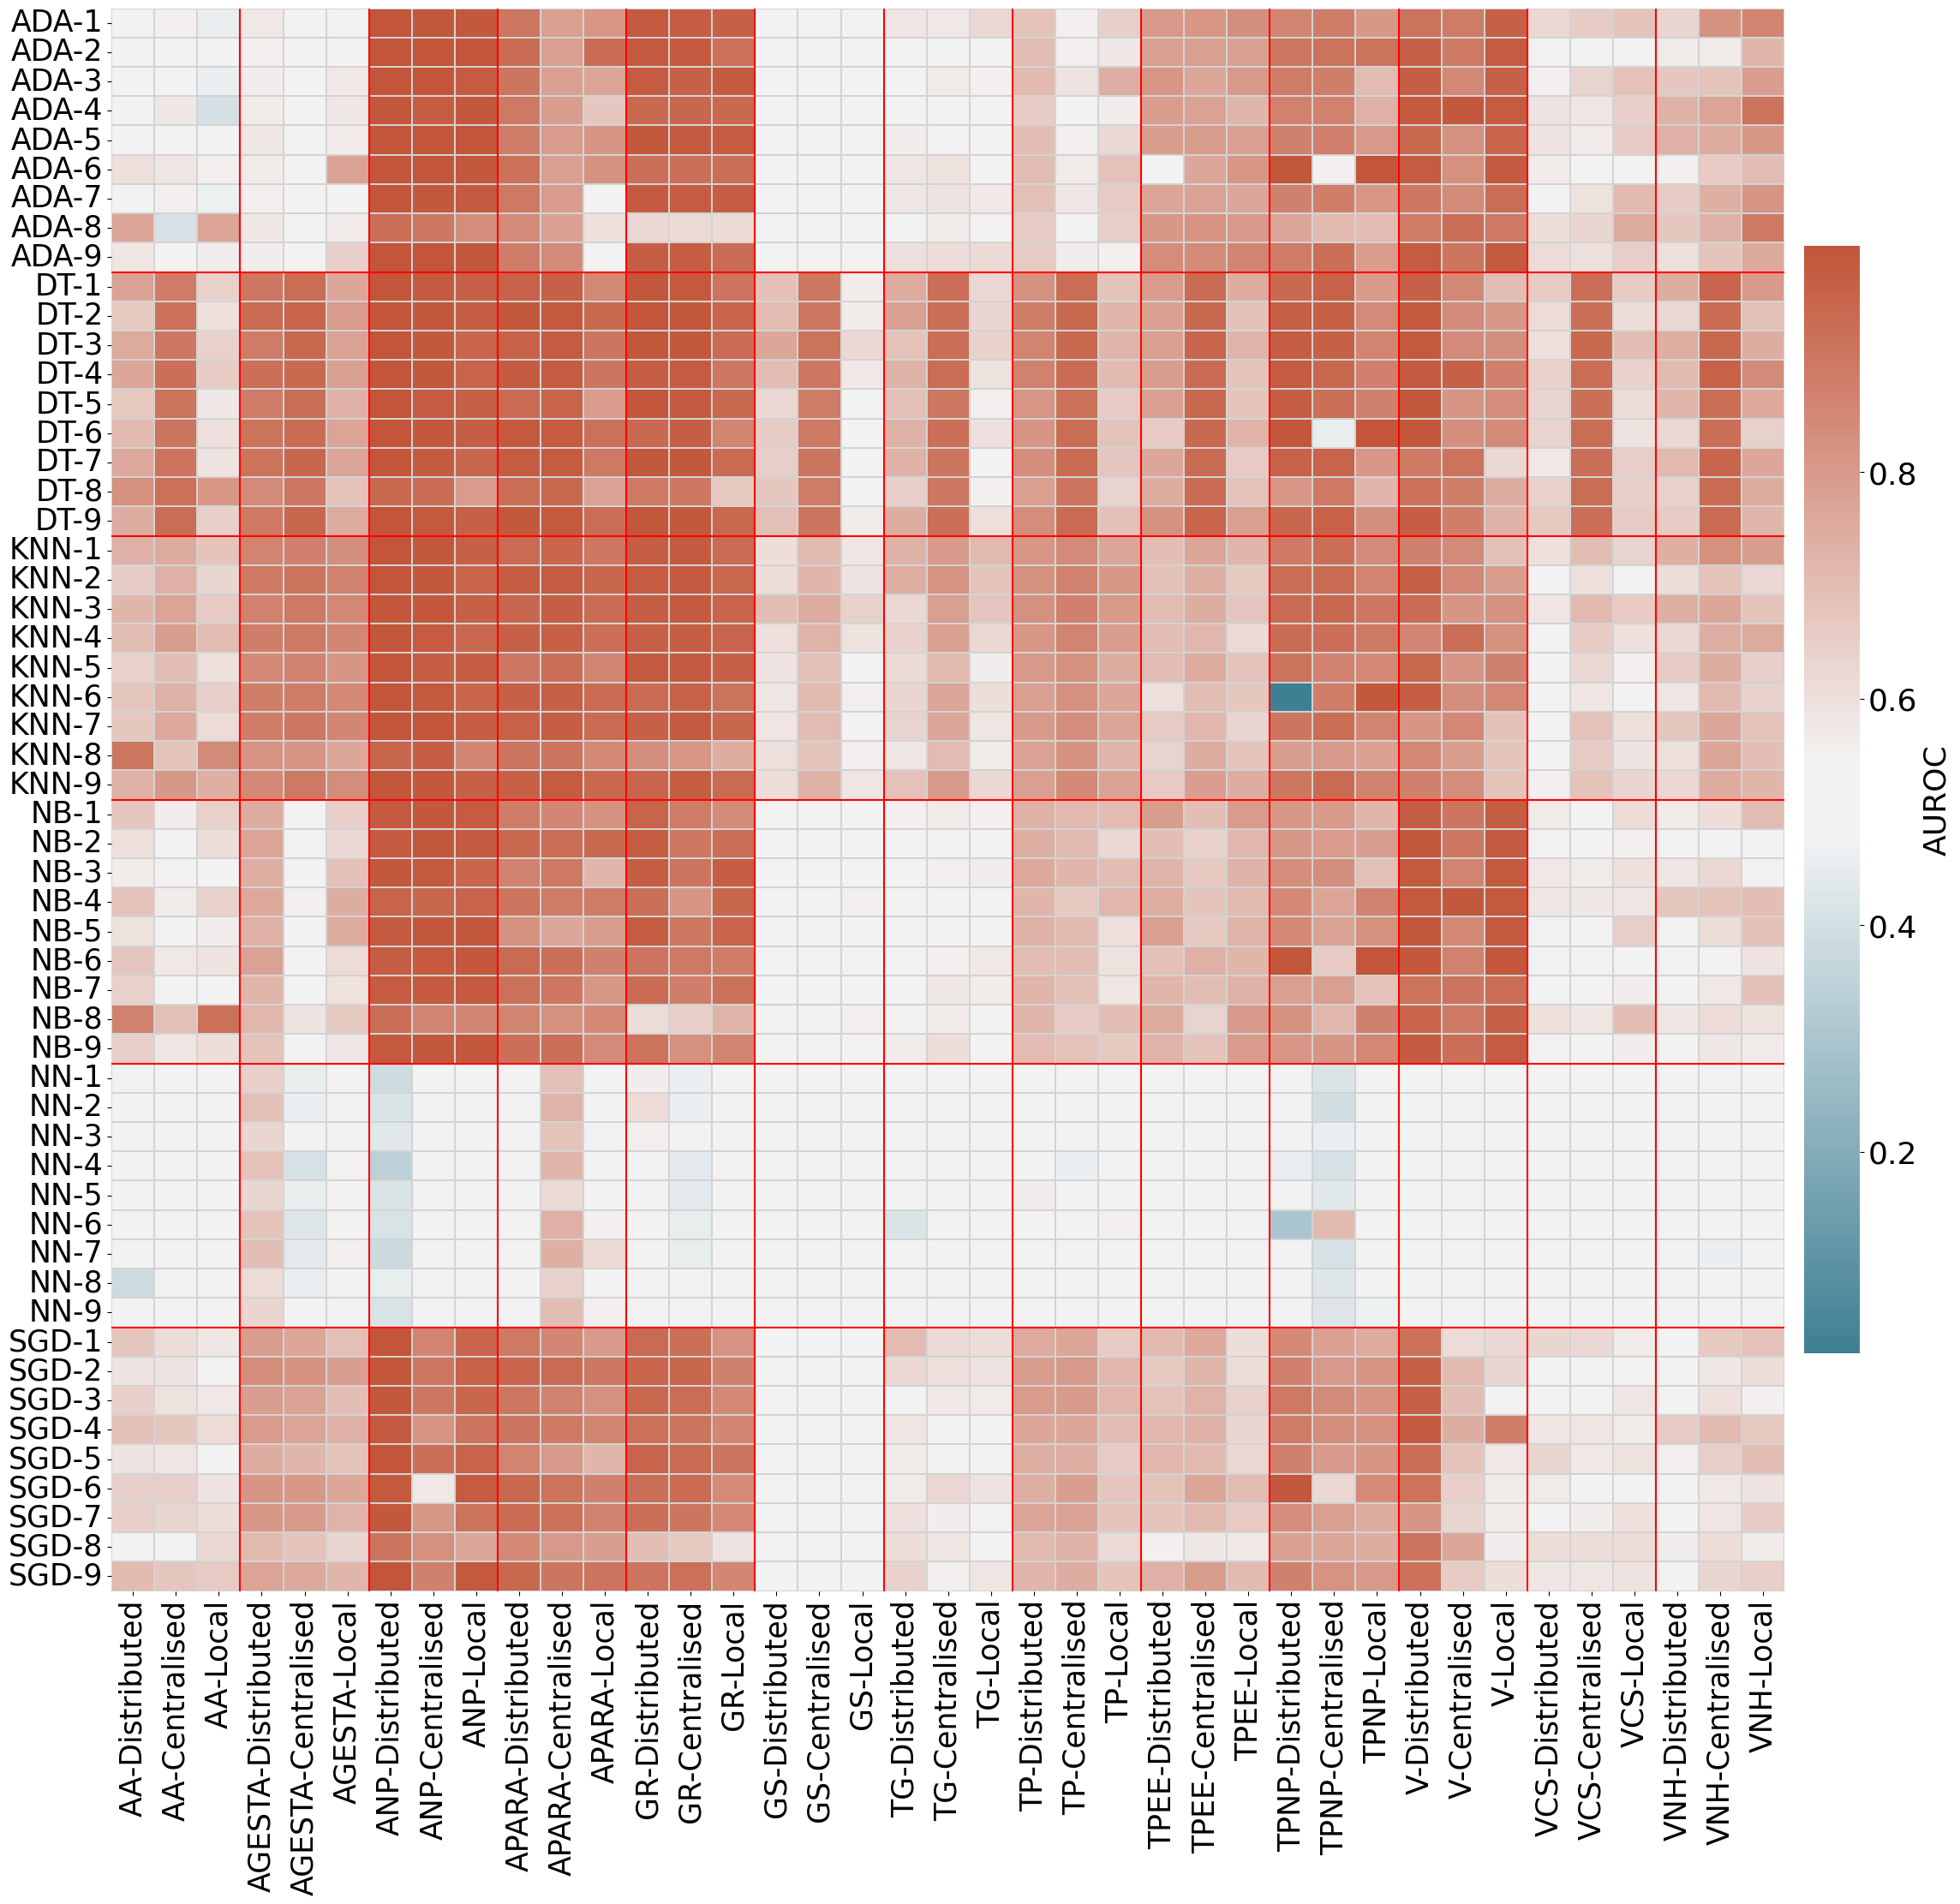
\includegraphics[scale=0.22]{figures/heatmap-class.png}
\end{figure}
%TC:endignore
%TC:ignore

\begin{figure}[htbp]
\centering
\captionsetup{justification=centering}

\caption[Heatmap of regression algorithm and silo vs Target variable and model type.]{Heatmap of regression algorithm and silo vs Target variable and model type. Value is the MAE mean of all 10 experiments. The y axis is the algorithm and silo. X axis is Target variable and Method. IA - Mother Age; IGA - Weeks on Admission; IMC - BMI; NRCPN - Nr of consultations; PI - Weight start of pregnancy; SGP - Weeks on Delivery;}\label{fig:heatmpa-int} 
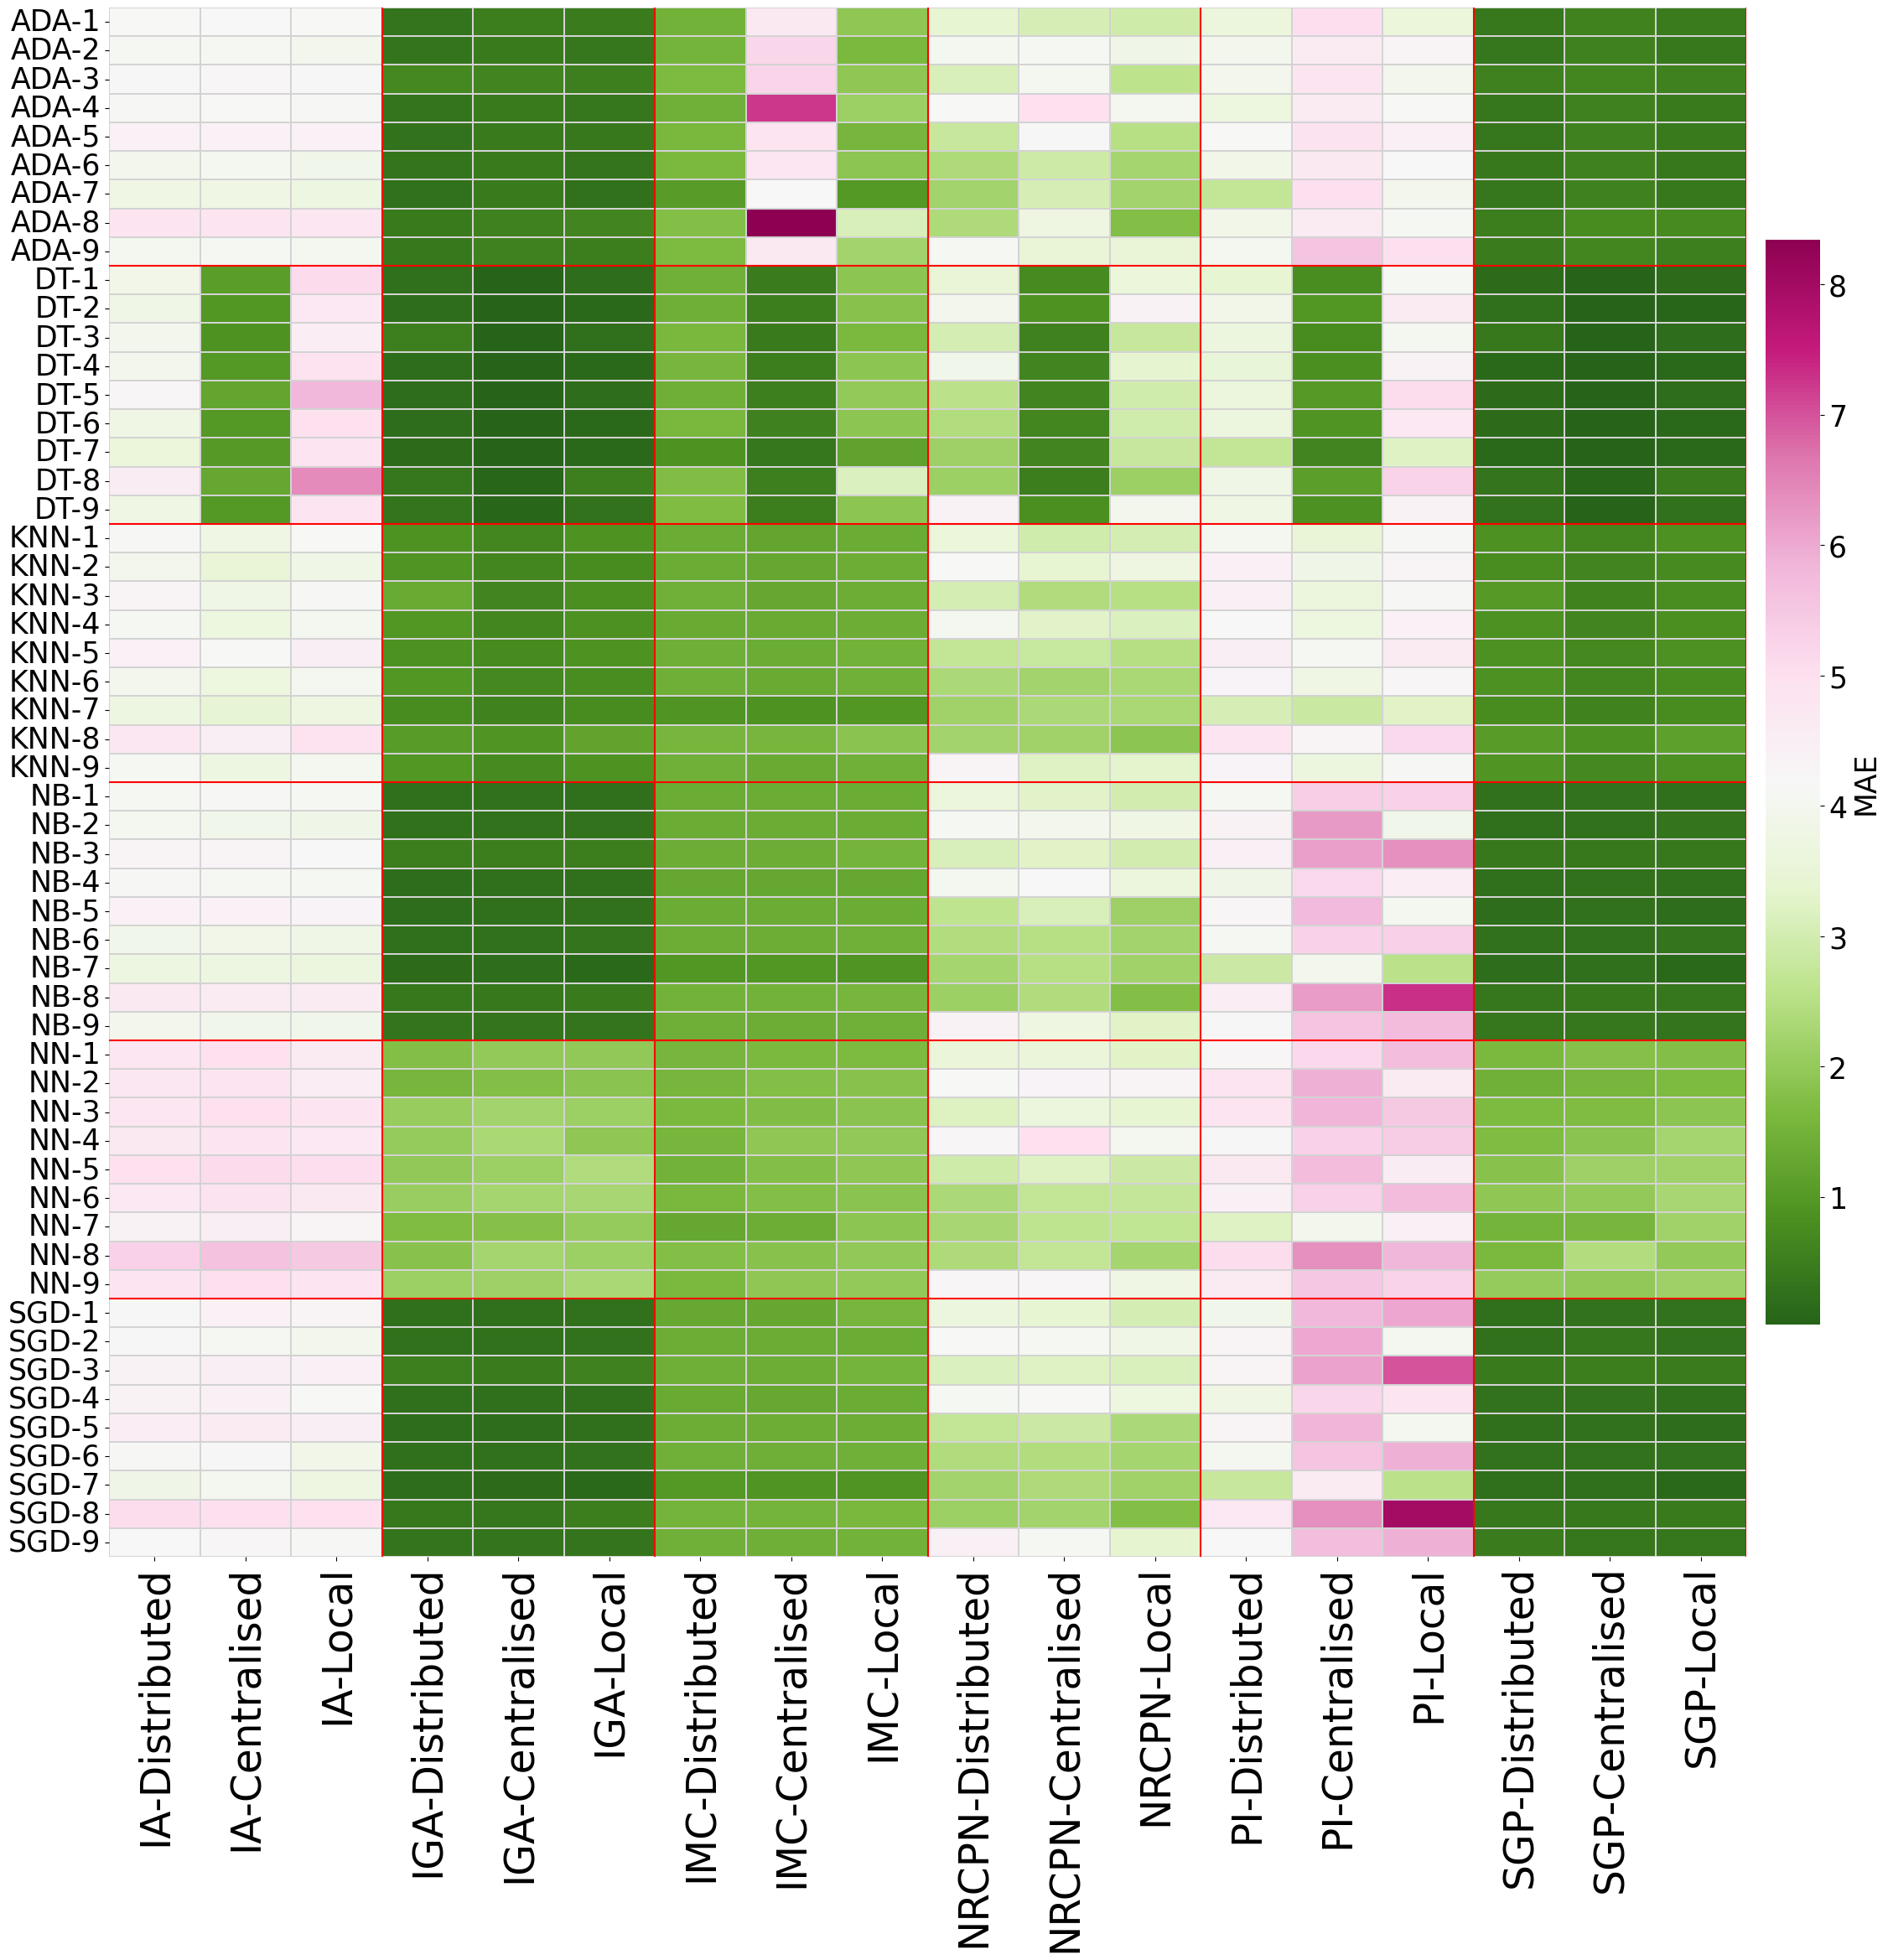
\includegraphics[scale=0.22]{figures/heatmap-reg.png}
\end{figure}
%TC:endignore

{\small
\definecolor{Gray}{gray}{0.85} 
 \begin{table}[h] 
 \setlength{\tabcolsep}{6pt} % Default value: 6pt 
 \renewcommand{\arraystretch}{1.1} % Default value: 1
  \captionsetup{justification=centering} 
\centering
\caption[Model comparison: Distributed versus centralised and local for every test]{Model comparison: Distributed versus centralised and local for every test. Each cell is the total of distributed model when compared with centralised model (row) and local model (column) across different silos and outcome variable. ($>$ for better, = for non significance and $<$ for worse). The first example is 72 which means that 72 iterations of the distributed SGD was better than the centralised and local. SGD: Stochastic Gradient Descent, NN: Neural Network, KNN: K-Nearest Neighbors, ADA: AdaBoost, NB: Naive Bayes, DT: Decision Tree. Comparison was done with 2-sample T-test with a $\alpha$ of 0.05. (\% in parentheses)}
\label{tab:hyp}
\begin{tabular}{llrrrr}
\toprule


 &  & Distributed $>$ Local & Distributed = Local & Distributed $<$ Local & \textbf{Row Total} \\


\hline \multirow{3}{*}{SGD} &Distributed $>$ Centralised  & 72 (7.0) & 14 (1.4) & 9 (0.8) & \textbf{95 (9.3)} \\
 & Distributed =  Centralised& 14 (1.4) & 17 (1.7) & 6 (0.6) & \textbf{37 (3.6) } \\
 & Distributed $<$ Centralised  & 11 (1.1) & 11 (1.1) & 17 (1.7) & \textbf{39 (3.8)} \\
% \hline
% \multicolumn{2}{c|}{SGD Total} & 97 (9.4)&42 (4.1) &32 (18.7)& \textbf{171}  \\
\hline \multirow{3}{*}{NN} & Distributed $>$ Centralised & 44 (4.3) & 44 (4.3) & 7 (0.7) & \textbf{95 (9.3)} \\
 & Distributed =  Centralised& 2 (0.2) & 33 (3.2) & 2 (0.2) & \textbf{37 (3.6)} \\
 & Distributed $<$ Centralised & 0 (0) & 17 (1.7) & 22 (2.1) & \textbf{39 (3.8)} \\
% \hline

% \multicolumn{2}{c|}{NN Total} & 46&94 &31 & \textbf{171}  \\

\hline \multirow{3}{*}{KNN} & Distributed $>$ Centralised & 16 (1.6) & 0 (0) & 1 (0.1) & \textbf{17 (1.7)} \\
 & Distributed =  Centralised & 10 (1) & 2 (0.2) & 1 (0.1) & \textbf{13 (1.3)} \\
 & Distributed $<$ Centralised & 72 (7)  & 28 (2.7) & 41 (4) & \textbf{141 (13.7)} \\
% \hline

% \multicolumn{2}{c|}{KNN Total} & 97&30 &43 & \textbf{171}  \\

\hline \multirow{3}{*}{ADA} & Distributed $>$ Centralised & 64 (6.2) & 25 (2.4) & 22 (2.1) & \textbf{111 (10.8)} \\
 & Distributed =  Centralised& 5 (0.5) & 12 (1.2) & 10 (1) & \textbf{27(2.6)} \\
 & Distributed $<$ Centralised & 10 (1) & 6 (0.6) & 17 (1.7) & \textbf{33 (3.2)} \\
% \hline

% \multicolumn{2}{c|}{ADA Total} & 79&43 &49 & \textbf{171}  \\

\hline \multirow{3}{*}{NB} & Distributed $>$ Centralised & 51 (5) & 19 (1.9) & 34 (3.3) & \textbf{104 (10.1) } \\
 &  Distributed =  Centralised & 5 (0.5) & 19 (1.9) & 12 (1.2) & \textbf{36 (3.5)} \\
 & Distributed $<$ Centralised  & 3 (0.3) & 4 (0.4) & 24 (2.3) & \textbf{31 (3)} \\
% \hline

% \multicolumn{2}{c|}{NB Total} & 59&42 &70 & \textbf{171}  \\

\hline \multirow{3}{*}{ DT} & Distributed $>$ Centralised & 27 (2.6) & 0 (0) & 1 (0.1) & \textbf{28 (2.7)} \\
 & Distributed = Centralised & 8 (0.8) & 0 (0) & 0 (0)& \textbf{8 (0.8)} \\
 & Distributed $<$ Centralised & 97 (9.5) & 12 (1.2) & 26 (2.5) & \textbf{135 (13.2)} \\
% \hline

% \multicolumn{2}{c|}{DT Total} & 132&12 &27 & \textbf{171}  \\
 
 \hline
  \textbf{Total} &  & \textbf{511 (49.8)} & \textbf{263 (25.6)} & \textbf{252 (24.6)} & \textbf{1026 (100)}\\
 \bottomrule
\end{tabular}
\end{table}
}
















\subsection{Discussion}
% !TeX root = ../../thesis.tex



A significant finding is that nearly 59\% of distributed models demonstrated comparable, if not superior, performance relative to their centralised counterparts (table \ref{tab:hyp} last column, first two values for each algorithm). From these, 41.9\% were also better or equal to the local model. If we take the best performing algorithm (SGD), we have 77.2\% for distributed better than centralised and 66\% better than centralised and local. This outcome underlines the potential of distributed models to offer reliable inference capabilities that match those of traditional centralised models, without sacrificing predictive accuracy. Furthermore, the adoption of distributed models enhances privacy for data owners, presenting a compelling case for their broader application in data-sensitive environments. Overall, our results suggest that it is possible to implement a distributed model without significantly losing information. Our analysis suggests that SGD, Adaboost and Naive Bayes approaches are suitable for such distributed approached with tabular data. However, MLPerceptron, Decision Trees and \ac{knn} do not seem to be a good approach for such use cases.

However, there are still issues to be addressed. This methodology presents hurdles regarding categorical class handling. Firstly, all classes should be known first-hand and should be given to each model even if that silo in particular has no cases of that class. Secondly, low-frequency classes are also an issue to be addressed, since training the model with cross-validation will raise problems because each split should have all classes present. Our approach relied on sample creation for low and non-existent target classes. However, this approach is adding information to the model that is not originally there. The way we chose for minimising this issue was by creating dummy variables with median and mode imputations based only on the information in the dataset. Nevertheless, non-existent classes are impossible to address without prior information. These class problems could be partially tackled in production by implementing data management and governance procedures, namely data dictionaries. Still on data preprocessing, we applied ordinal encoding to the variables which will create a natural hierarchy between variables. One solution for this is to create binary columns for each class in each column. This will remove the hierarchy between classes but increase variable numbers and training time considerably.\\

Another issue to consider is the path adopted to build the distributed model. In this case, it was decided to develop an ensemble of models with voting. However, other methods could have been employed, like parameter averaging, that should be tested as well. In particular, the usage of more robust neural networks could be assessed as well. We chose not to test state-of-the-art neural networks since the data volume was low for that use case and several papers have already demonstrated that neural networks are not the most suitable tool for tabular data \cite{grinsztajnWhyTreebasedModels2022,borisovDeepNeuralNetworks2022}. We chose to add MLPerceptron as a baseline for comparison with the remaining algorithms. The results show us that the performance was below the other algorithms, but in this concrete case, the problem may reside in the architecture chosen and hyperparameters used in the Cross-validation which may have lead to underfitting. Despite this, a precise and thorough demonstration of this use case would be important to consider such scenarios. \\
Furthermore, the algorithm underlying the distributed model is of importance as well for its performance versus the centralised model. Figures \ref{fig:heatmap-cat} and \ref{fig:heatmpa-int} and table \ref{tab:hyp} show us that Decision trees and \ac{knn} implemented in a centralised manner are consistently better than the distributed counterpart. This is specially notorious in the case of the decision trees. We believe this may be related to way the algorithm is implemented. A centralised version may be able to create optimal splits in the data, while the distributed version may not be able to do so. This is a topic that should be further explored.\\
Even though this improvement may have a relationship to the target variable (i.e. figure \ref{fig:heatmpa-int} for IA and IGA variables), it is still an important fact to take into account when implementing such architectures.
The performance of the models is also interesting to catch differences in silos. See silo 6 for TPNP (figure \ref{fig:heatmap-cat}) where silo 6 consistently behaves differently than the rest.
Checking performance data regarding regression tasks, we can see a drop in performance for PI and IA. While the explanation for the performance of IA can be explained by the average value of it which is 66. This is the highest average in the dataset. This means that the model will have a harder time predicting these values. This is also true for the distributed model. This is a topic that should be further explored.\\
As for implementation, such a mechanism could be implemented in at least two manners; with a central orchestrator or without. The first one would assume a central point that would make a request to each silo for a prediction and then create the final prediction with the weighted averaging of each one. The second one would not require any additional platform and each silo would communicate with each of the others and receive the prediction and would create the final with their own. This implementation step would of course take into account variables that we were out of scope such as the communication between silos. 
Regarding the prediction capability as a whole, we found that this data is suitable to apply machine-learning models in order to predict several clinical outcomes, with very good results for several target variables. 


\subsection{Conclusion}
Bud1hh` 0x8 OBS  @� @� @� @$imagens-tese.jpgIlocblob���������imagens-tese.pptxIlocblob����������LivrosIlocblob����������Livrosbwspblob�bplist00�	]ShowStatusBar[ShowToolbar[ShowTabView_ContainerShowSidebar\WindowBounds[ShowSidebar			_{{-1920, 0}, {1728, 1055}}	#/;R_klmno�
�LivrosvSrnlongmetadata Sonho.xlsxIlocblobA&������
NewsletterIlocblob�&��������
obs-cdss-fhirIlocblob&������
obs-model.pngIlocblob.������Outras apresentac'oesIlocblob�&��������Outras apresentac'oesbwspblob�bplist00�	]ShowStatusBar[ShowToolbar[ShowTabView_ContainerShowSidebar\WindowBounds[ShowSidebar			_{{-1920, 0}, {1920, 1055}}	#/;R_klmno�
�Outras apresentac'oeslg1ScompOutras apresentac'oesmoDDblob�[�&��AOutras apresentac'oesmodDblob�[�&��AOutras apresentac'oesph1ScompOutras apresentac'oesvSrnlongPapersIlocblob�&��������Papersbwspblob�bplist00�	]ShowStatusBar[ShowToolbar[ShowTabView_ContainerShowSidebar\WindowBounds[ShowSidebar			_{{272, -208}, {1920, 1055}}	#/;R_klmno�
�PapersvSrnlongpesquisas pubmed.xlsxIlocblobg&��������Report teseIlocblob�������Report tesebwspblob�bplist00�	]ShowStatusBar[ShowToolbar[ShowTabView_ContainerShowSidebar\WindowBounds[ShowSidebar			_{{0, 0}, {1920, 1055}}	#/;R_klmno�
�Report teselg1ScompReport tesemoDDblob���+�0�AReport tesemodDblob���+�0�AReport teseph1ScompReport tesevSrnlong
response.docxIlocblob�������response.pdfIlocblob��������	reunioesIlocblob��������	reunioesbwspblob�bplist00�	]ShowStatusBar[ShowToolbar[ShowTabView_ContainerShowSidebar\WindowBounds[ShowSidebar			_{{-1636, 161}, {1186, 604}}	#/;R_klmno�
�	reunioesvSrnlongreviewsIlocblob��������reviewsbwspblob�bplist00�	]ShowStatusBar[ShowToolbar[ShowTabView_ContainerShowSidebar\WindowBounds[ShowSidebar			_{{-1920, 0}, {1920, 1055}}	#/;R_klmno�
�reviewsvSrnlongtitle-page.docxIlocblob��������0. thesis-supportIlocblobA.��������1. repositorio de dadosIlocblob�.������2. dados sinteticosIlocblob.������2. dados sinteticosbwspblob�bplist00�	]ShowStatusBar[ShowToolbar[ShowTabView_ContainerShowSidebar\WindowBounds[ShowSidebar			_{{2228, 501}, {920, 436}}	#/;R_klmno�
�2. dados sinteticosvSrnlong2.1 pedidos instituic'oesIlocblob�.��������2.1 pedidos instituic'oesbwspblob�bplist00�	]ShowStatusBar[ShowToolbar[ShowTabView_ContainerShowSidebar\WindowBounds[ShowSidebar			_{{452, 125}, {1220, 709}}	#/;R_klmno�
�2.1 pedidos instituic'oesvSrnlong3.1 survey GANIlocblob�.������3.1 survey GANbwspblob�bplist00�	]ShowStatusBar[ShowToolbar[ShowTabView_ContainerShowSidebar\WindowBounds[ShowSidebar			_{{179, 121}, {1186, 604}}	#/;R_klmno�
�3.1 survey GANvSrnlong3.2 phd consortium aimeIlocblobg.������3.4 survey fullIlocblobA�������3.6 distributed learningIlocblob����������3.6 distributed learningbwspblob�bplist00�]ShowStatusBar[ShowToolbar[ShowTabView_ContainerShowSidebar\WindowBounds[ShowSidebar				_{{0, 0}, {1728, 1055}}	#/;R_klmno�
�3.6 distributed learningicvpblob�bplist00�	

_backgroundColorBlueXiconSizeXtextSize_backgroundColorRed^backgroundType_backgroundColorGreen[gridOffsetX_scrollPositionY[gridOffsetY\showItemInfo_viewOptionsVersion_scrollPositionXYarrangeBy]labelOnBottom_showIconPreview[gridSpacing#?�#@P#@(#Tnone		#@K+AJShw��������"+4=?HIZ_`aj3.6 distributed learningvSrnlong3.7 analise dadosIlocblob�������3.7 analise dadosbwspblob�bplist00�	]ShowStatusBar[ShowToolbar[ShowTabView_ContainerShowSidebar\WindowBounds[ShowSidebar			_{{179, 121}, {1186, 604}}	#/;R_klmno�
�3.7 analise dadosvSrnlong
3.8 OBS MLIlocblob����������
3.8 OBS MLbwspblob�bplist00�	]ShowStatusBar[ShowToolbar[ShowTabView_ContainerShowSidebar\WindowBounds[ShowSidebar			_{{0, 0}, {1728, 1055}}	#/;R_klmno�
�
3.8 OBS MLicvpblob�bplist00�	

_backgroundColorBlue_showIconPreviewXtextSize_backgroundColorRed^backgroundType_backgroundColorGreen[gridOffsetX_scrollPositionY[gridOffsetY\showItemInfo_viewOptionsVersion_scrollPositionXYarrangeBy]labelOnBottomXiconSize[gridSpacing#?�	#@(#\dateModified	#@P#@K+AS\q���������
"+,57@AR_`ir
3.8 OBS MLlsvpblob�bplist00�	

HIJKMXiconSize_showIconPreviewWcolumns_calculateAllSizes_scrollPositionYXtextSize_scrollPositionXZsortColumn_useRelativeDates_viewOptionsVersion#@0	� %*/48=BXcommentsUlabelWversion[dateCreatedTsize\dateModifiedTkindTname^dateLastOpened�UindexUwidthYascendingWvisible,	�!"d	�&'K	�+,��01a	�5,	�9:s		�>?:		�CD�#@3#@*#Tname	&8@Tfo������������(.4>FHKLMVXZ[\egijktvxyz������������������������������N�
3.8 OBS MLvSrnlong3.9 Catalogar DatasetIlocblob����������3.9 Catalogar Datasetbwspblob�bplist00�	]ShowStatusBar[ShowToolbar[ShowTabView_ContainerShowSidebar\WindowBounds[ShowSidebar			_{{-1516, 283}, {1206, 635}}	#/;R_klmno�
�3.9 Catalogar Dataseticvpblob�bplist00�	

_backgroundColorBlue_showIconPreviewXtextSize_backgroundColorRed^backgroundType_backgroundColorGreen[gridOffsetX_scrollPositionY[gridOffsetY\showItemInfo_viewOptionsVersion_scrollPositionXYarrangeBy]labelOnBottomXiconSize[gridSpacing#?�	#@(#Tnone	#@P#@K+AS\q���������
"+,57@ARWXaj3.9 Catalogar Datasetlg1Scomp3.9 Catalogar DatasetmoDDblobZ$8����A3.9 Catalogar DatasetmodDblobZ$8����A3.9 Catalogar Datasetph1Scomp3.9 Catalogar DatasetvSrnlong4.0 IPOPIlocblobg�������4.0 IPOPbwspblob�bplist00�	]ShowStatusBar[ShowToolbar[ShowTabView_ContainerShowSidebar\WindowBounds[ShowSidebar			_{{0, 0}, {1920, 1055}}	#/;R_klmno�
�4.0 IPOPicvpblob�bplist00�	

_backgroundColorBlue_showIconPreviewXtextSize_backgroundColorRed^backgroundType_backgroundColorGreen[gridOffsetX_scrollPositionY[gridOffsetY\showItemInfo_viewOptionsVersion_scrollPositionX]labelOnBottomYarrangeByXiconSize[gridSpacing#?�	#@(#	Tnone#@P#@K+AS\q��������
"+,57@ARSXaj4.0 IPOPvSrnlong5.0 historia SISIlocblobA*��������6.0 logs HospitaisIlocblob�*������6.0 logs Hospitaisbwspblob�bplist00�	]ShowStatusBar[ShowToolbar[ShowTabView_ContainerShowSidebar\WindowBounds[ShowSidebar			_{{-1920, 0}, {1920, 1055}}	#/;R_klmno�
�6.0 logs Hospitaisicvpblob�bplist00�	

_backgroundColorBlue[gridSpacingXtextSize_backgroundColorRed^backgroundType_backgroundColorGreen[gridOffsetX_scrollPositionY[gridOffsetY\showItemInfo_viewOptionsVersion_scrollPositionXYarrangeBy]labelOnBottomXiconSize_showIconPreview#?�#@K#@(#Tnone	#@P	+AMVkz��������"+4=?HIZ_`ij6.0 logs HospitaisvSrnlong7.0 Data qualityIlocblob*��������7.0 Data qualitybwspblob�bplist00�	]ShowStatusBar[ShowToolbar[ShowTabView_ContainerShowSidebar\WindowBounds[ShowSidebar			_{{0, 0}, {1728, 1055}}	#/;R_klmno�
�7.0 Data qualitylsvCblob5bplist00�	

TUVWX_viewOptionsVersion_showIconPreviewWcolumns_calculateAllSizes_scrollPositionYXtextSize_scrollPositionXZsortColumnXiconSize_useRelativeDates	�!%*/49=BFJN�WvisibleUwidthYascendingZidentifier	,	Tname�Xubiquity#� 	�\dateModified�$[dateCreated�')	aTsize�,.	s	Tkind�13d	Ulabel�68K	Wversion�<	Xcomments�?A�^dateLastOpened�?EZshareOwner�?I_shareLastEditor�KYdateAdded�PR�_invitationStatus#@G�#@*#Tname#@0	2DL`r{����������� !*+-.;DEFR[\^_dmnpqv�������������������������
 "#67@IRW`Za7.0 Data qualitylsvpblob�bplist00�	

GHIJK_viewOptionsVersion_showIconPreviewWcolumns_calculateAllSizes_scrollPositionYXtextSize_scrollPositionXZsortColumnXiconSize_useRelativeDates	� %*/48=AXcommentsUlabelWversion[dateCreatedTsize\dateModifiedTkindTname^dateLastOpened�UindexUwidthYascendingWvisible,	�!"d	�&'K	�+,��01a	�5,	�9:s		�>		�BC�#@G�#@*#Tname#@0	2DL`r{�����������'06<FNPSTU^`bcdmoqrs|~��������������������������������M�7.0 Data qualityvSrnlong8.0 dataset similarityIlocblob�*��������8.0 dataset similaritybwspblob�bplist00�	]ShowStatusBar[ShowToolbar[ShowTabView_ContainerShowSidebar\WindowBounds[ShowSidebar			_{{-1654, 142}, {1091, 843}}	#/;R_klmno�
�8.0 dataset similaritylsvCblob*bplist00�	

TUTVXXiconSize_showIconPreviewWcolumns_calculateAllSizes_scrollPositionYXtextSize_scrollPositionXZsortColumn_useRelativeDates_viewOptionsVersion#@0	�!%*/49=BFJN�ZidentifierYascendingUwidthWvisibleTname	,	�Xubiquity#�\dateModified�	�"[dateCreated�&(Tsizea	�+-Tkind	s	�02Ulabel	d�57Wversion	K�:Xcomments	�>@^dateLastOpened��C@ZshareOwner�G@_shareLastEditor�KYdateAdded�PR�_invitationStatus##@*Tname	&8@Tfo��������������"/023<HIJSXY[\ejkmnw}~������������������������
./8AFGYX8.0 dataset similaritylsvpblob�bplist00�	

GHGIKXiconSize_showIconPreviewWcolumns_calculateAllSizes_scrollPositionYXtextSize_scrollPositionXZsortColumn_useRelativeDates_viewOptionsVersion#@0	� %*/48=AXcommentsUlabelWversion[dateCreatedTsize\dateModifiedTkindTname^dateLastOpened�WvisibleYascendingUwidthUindex	,�#$	d�()	K�-.��23	a�-7	�;<		s�@		�DE�##@*Tname	&8@Tfo������������(0:@FGHKMVWXZ\efgiktuvxz����������������������������L�8.0 dataset similarityvSrnlong9.0 benchmark clusterIlocblob�*������9.0 benchmark clusterbwspblob�bplist00�	]ShowStatusBar[ShowToolbar[ShowTabView_ContainerShowSidebar\WindowBounds[ShowSidebar			_{{211, 219}, {1186, 604}}	#/;R_klmno�
�9.0 benchmark clustervSrnlong99. Process MiningIlocblobg*������99. Process MiningvSrnlong-Captura de ecra 2023-12-06, as 16.25.16.pngIlocblob�.������-Captura de ecra 2023-12-06, as 16.25.26.pngIlocblobC.������-Captura de ecra 2024-02-26, as 10.44.33.pngIlocblob�.������1Captura de ecra 2024-03-26, as 14.13.56 (2).pngIlocblob�.������-Captura de ecra 2024-03-26, as 14.14.05.pngIlocblobi.������-Captura de ecra 2024-03-26, as 14.16.27.pngIlocblob��������clinical_assessment.pngIlocblob�.������dec-tese-rjc.pdfIlocblobC�������DocsIlocblobA���������Docsbwspblob�bplist00�	]ShowStatusBar[ShowToolbar[ShowTabView_ContainerShowSidebar\WindowBounds[ShowSidebar			_{{0, 0}, {1920, 1055}}	#/;R_klmno�
�DocsvSrnlongExemplos outras pessoasIlocblob��������Exemplos outras pessoasbwspblob�bplist00�	]ShowStatusBar[ShowToolbar[ShowTabView_ContainerShowSidebar\WindowBounds[ShowSidebar			_{{490, 144}, {1091, 843}}	#/;R_klmno�
�Exemplos outras pessoaslg1ScompExemplos outras pessoasmoDDblob��b3�AExemplos outras pessoasmodDblob��b3�AExemplos outras pessoasph1ScompExemplos outras pessoasvSrnlongFinalIlocblobC������heads-thesisIlocblob��������heads-thesisbwspblob�bplist00�	]ShowStatusBar[ShowToolbar[ShowTabView_ContainerShowSidebar\WindowBounds[ShowSidebar			_{{2420, 422}, {920, 492}}	#/;R_klmno�
�heads-thesislsvCblob:bplist00�	

UVWXZXiconSize_showIconPreviewWcolumns_calculateAllSizes_scrollPositionYXtextSize_scrollPositionXZsortColumn_useRelativeDates_viewOptionsVersion#@0	�!%*/49>CGKO�ZidentifierUwidthYascendingWvisibleTname0		�Xubiquity#�\dateModified�	�"[dateCreated�&'Tsizea	�+,Tkinds		�01Ulabeld	�56WversionK	�:;Xcomments,	�?@^dateLastOpened��D@ZshareOwner�H@_shareLastEditor�LYdateAdded�QS�_invitationStatus#@a`#@*#Tname	&8@Tfo�������������"/123<HIJSXZ[\ejlmnw}�������������������������12;DMRS[dheads-thesislsvpblob�bplist00�	

HIJKMXiconSize_showIconPreviewWcolumns_calculateAllSizes_scrollPositionYXtextSize_scrollPositionXZsortColumn_useRelativeDates_viewOptionsVersion#@0	� %*/48=BXcommentsUlabelWversion[dateCreatedTsize\dateModifiedTkindTname^dateLastOpened�WvisibleUwidthYascendingUindex,	�"$d	�')K	�,.��13	a�,7	�:<	s	�?A	0	�DF�#@a`#@*#Tname	&8@Tfo������������(06@FGJKMVWYZ\efhiktuwxz������������������������������N�	]ShowStatusBar[ShowToolbar[ShowTabView_ContainerShowSidebar\WindowBounds[ShowSidebar			_{{211, 219}, {1186, 604}}	#/;R_klmno�
�9.0 benchmark clustervSrnlong99. Process MiningIlocblobg*������
3.8 OBS MLlsvCblob:bplist00�	

UVWXZXiconSize_showIconPreviewWcolumns_calculateAllSizes_scrollPositionYXtextSize_scrollPositionXZsortColumn_useRelativeDates_viewOptionsVersion#@0	�!%*/49>CGKO�WvisibleUwidthYascendingZidentifier	:	Tname�#Xubiquity� 	�\dateModified�$[dateCreated�')	aTsize�,.	s	Tkind�13d	Ulabel�68K	Wversion�;=,	Xcomments�@B�^dateLastOpened�@FZshareOwner�@J_shareLastEditor�NYdateAdded�PQ_invitationStatus�#@3#@*#Tname	&8@Tfo���������������
"#%&3<=>JSTVW\efhinwxz{������������������������-/012;DMRS[d7.0 Data qualityicvpblob�bplist00�	

_backgroundColorBlue[gridSpacingXtextSize_backgroundColorRed^backgroundType_backgroundColorGreen[gridOffsetX_scrollPositionY[gridOffsetY\showItemInfo_viewOptionsVersion_scrollPositionXYarrangeBy]labelOnBottom_showIconPreviewXiconSize#?�#@K#@(#Tnone		#@P+AMVkz��������"+4=?HIZ_`aj99. Process Miningbwspblob�bplist00�	]ShowStatusBar[ShowToolbar[ShowTabView_ContainerShowSidebar\WindowBounds[ShowSidebar			_{{138, 192}, {920, 492}}	#/;R_klmno�
�heads-thesisvSrnlongb��b3�AExemplos outras pessoasmodDblob��b3�AExemplos outras pessoasph1ScompExemplos outras pessoasvSrnlongFinalIlocblobC������heads-thesisIlocblob��������heads-thesisbwspblob�bplist00�	]ShowStatusBar[ShohE` 0@PDSDB `�p� @� @Tnone		#@P+AMVkz��������"+4=?HIZ_`aj99. Process Miningbwspblob�bplist00�	]ShowStatusBar[ShowToolbar[ShowTabView_ContainerShowSidebar\WindowBounds[ShowSidebar			_{{138, 192}, {920, 492}}	#/;R_klmno�
�heads-thesisvSrnlongb��b3�AExemplos outras pessoasmodDblob��b3�AExemplos outras pessoasph1ScompExemplos outras pessoasvSrnlongFinalIlocblobC������heads-thesisIlocblob��������heads-thesisbwspblob�bplist00�	]ShowStatusBar[Sho


\section{Can Institutions Share Their Performance Metrics Without Hesitation of Retaliation?}\label{subsec:benchmark}
This section is based on the paper entitled "Benchmarking institutions' health outcomes with clustering methods" (in review). This paper was focused on the fact that many healthcare institutions harbour reservations about openly sharing production metrics. One predominant concern is the potential for retaliatory actions, be it from regulatory bodies, competitors, or the public. In this paper, we propose the application of a clustering methodology that allows institutions to compare performance metrics without disclosing the actual values. The method is based on clustering, which involves grouping health institutions' outcomes into a known number of clusters, allowing institutions to position themselves in a range of clusters without sharing the true means of their target data. The proposed method uses the K-means and K-modes clustering algorithms and was tested on data from real Electronic health records and public datasets. This approach provides a valid benchmark of hospital metrics and performances while protecting the privacy of participating institutions. 
\subsection{Introduction}
Health institutions play a critical role in providing essential healthcare services to communities and ensuring that they operate efficiently and effectively is crucial. Benchmarking is a process that allows hospitals to compare their performance against that of other institutions, which can help identify areas of strength and weakness \cite{suydamPatientSafetyData2007}. By analyzing and evaluating performance metrics, such as patient outcomes, operational efficiency, and financial management, hospitals can identify best practices and make data-driven decisions to improve their overall performance. It can also help hospitals identify and implement innovative practices that can lead to better patient care and improved staff satisfaction \cite{hulsenSharingCaringData2020}.

However, despite the numerous benefits of benchmarking, some hospitals may be hesitant to participate due to concerns about revealing weaknesses or being perceived as inferior to their peers. The fear of being judged or penalized for poor performance can sometimes lead hospitals to avoid sharing data, making it difficult to accurately assess their performance and identify areas for improvement. Privacy issues and concerns turn this opportunity into an even less desirable path \cite{hulsenSharingCaringData2020}. To address these concerns, benchmarking initiatives often ensure the confidentiality and anonymity of data to encourage participation and foster trust among participating institutions. However, this is usually not enough. In 2019, as stated in the work of Villanueva et al., \cite{villanuevaCharacterizingBiomedicalDataSharing2019}, 26\% of data-sharing initiatives are based on the aggregation of data and 24\% are based on sharing data in closed consortia. Only 15\% were based on open or controlled access.

To address concerns around privacy and confidentiality, we propose a new method of benchmarking based on clustering. This method involves grouping health institutions' outcomes into a known number of clusters, providing health institutions with the capability of positioning themselves in a range of clusters, without ever sharing the true means of their target data.

This approach to benchmarking not only addresses concerns around privacy and confidentiality. It has the potential to encourage greater participation in benchmarking initiatives, as hospitals can be assured of the anonymity and confidentiality of their data. By creating a more secure and private environment for benchmarking, hospitals can feel more comfortable sharing their data and participating in initiatives that can ultimately improve patient care and operational efficiency.

In conclusion, benchmarking is a crucial tool for hospitals to improve their performance and provide better care for their patients. While concerns around privacy and confidentiality may exist, the clustering approach to benchmarking provides a more accurate assessment of hospital performance while protecting the privacy of participating institutions. By embracing benchmarking initiatives and leveraging new approaches to benchmarking, hospitals can continuously improve their operations and ensure they provide the highest quality of care possible.
In this paper we propose:
\begin{myitemize}
    \item study how to implement clustering mechanism for benchmark
    \item address preprocessing issues for the raw data
    \item highlight pain points to deployment in the real world.
\end{myitemize}
\subsection{Rationale and Related Work}
This work was initially suggested as a follow-up to a previous work of Rodrigues et al., \cite{rodriguesLocalAlgorithmApproximate2018a} where clustering is applied to streaming data sources. We then thought if a similar approach could be applied to healthcare in order to be able to compare data distributions without ever knowing their real values of them.
Clustering in healthcare is often used to create clusters of patients, taking into account a given set of characteristics. This is used to find possible groups of phenotype and be able to characterise populations given the centroids \cite{walkerUnsupervisedLearningTechniques2019,basileInformaticsMachineLearning2018}. It is also used as a method of detecting regularities and patterns in multi-omics data that reveal different molecular subtypes \cite{nicoraIntegratedMultiOmicsAnalyses2020,rappoportMultiomicMultiviewClustering2018}. It can also be used to create unsupervised models for facilitating the annotation of data for supervised models \cite{mcalpineUtilityUnsupervisedMachine2022}. 

K-means \cite{lloydLeastSquaresQuantization1982,steinley2007initializing,macqueen1967classification} is an unsupervised clustering algorithm used to group data points into K distinct clusters based on their similarity. It is widely used in machine learning, data mining, and image segmentation. The algorithm works by randomly initializing K centroids (or cluster centres) and assigning each data point to the nearest centroid. Then, the centroids are moved to the mean of the points assigned to each cluster. This process is repeated until convergence, where the clusters no longer change.

The objective of K-means is to minimize the sum of squared distances between each data point and its assigned centroid, which is also called the within-cluster sum of squares (WCSS). The algorithm attempts to find the best K clusters that minimize the WCSS. However, choosing the right value of K can be challenging, and the algorithm may converge to a suboptimal solution. Therefore, K-means is often run multiple times with different initializations to find the best clustering solution. Despite its simplicity, K-means can be computationally expensive when dealing with large datasets, and it may not work well with non-linearly separable data or when the clusters have different shapes and sizes.

K-modes is another clustering algorithm similar to K-means, but it is designed to work with categorical data. Unlike K-means, which computes the mean of continuous variables, K-modes computes the mode (or the most frequent value) of categorical variables within each cluster. The algorithm works by randomly initializing K centroids and assigning each data point to the nearest centroid based on the number of matching categories. Then, the centroids are moved to the mode of the categories within each cluster. This process is repeated until convergence, where the clusters no longer change.

The objective of K-modes is to minimize the dissimilarity between the data points within each cluster, which is often measured by the Hamming distance, Jaccard distance, or other similarity measures. Like K-means, choosing the right value of K is critical, and the algorithm may converge to a suboptimal solution. Therefore, K-modes is often run multiple times with different initializations to find the best clustering solution. K-modes is particularly useful when dealing with data that have a large number of categorical variables or when the data contain missing values. However, like K-means, K-modes may not work well with non-linearly separable data or when the clusters have different shapes and sizes.

However, as far as we know, this is the first time clustering is tested for exchanging information privately.

\subsection{Materials \& Methods}

\subsubsection{Materials}
We used two types of data in this paper. One is simpler and available online from the \ac{uci} dataset library, namely, the heart disease dataset \cite{misc_heart_disease_45}. We made fairly simple preprocessing on that dataset, namely removing the "?" by filling with null and then imputing missing values by imputing the mean on continuous variables and mode on categorical ones. We then separated the data into 3 distinct silos at random to mimic different health institutions.

In order to use real data and address problems found in the wild, we used clinical data gathered from nine different Portuguese hospitals regarding obstetric information, pertaining to admissions from 2019 to 2020. This originated from nine different files representing different sets of patients but with the same features associated with them. The software for collecting data was the same in every institution (although different versions existed across hospitals) - ObsCare. The data columns are the same in every hospital's database. Each hospital was considered a silo for comparison.
\subsubsection{Method Overview}
We used Python 3.9 to implement the mock example of such an use-case. The clustering was done with scikit-learn library \cite{scikit-learn}. The algorithm proposed is shown in algorithm \ref{alg:bench1}.

%TC:ignore
\begin{algorithm}[hbtp]
\caption{Benchmarking with clustering}
\label{alg:bench1}

\SetAlgoLined



\For {variable in silo}{ 
initialize centroids\;
%\begin{itemize}
%    \item real cluster obfuscated with noise
%    \item true centroids
%    \item add noise to data and then create centroids
%\end{itemize}
}
%\SetKwRepeat{Do}{do}{while}
\While{No convergence}{
\begin{itemize}
    \item Send centroids to other silos
\item Receive other silo's information and add own centroids
\item Calculate new centroids
\item calculate score
\end{itemize}
}



\end{algorithm}
%TC:endignore

The method for assessing convergence is based on clustering metrics: the \ac{ri}. This metric computes a similarity measure between two clusters by considering all pairs of samples and counting pairs that are assigned in the same or different clusters in the predicted and true clusters \cite{hubertComparingPartitions1985}. The raw RI score is: $RI = (number\; of\; agreeing\; pairs) / (number\; of\; pairs)$.
Furthermore, convergence must be obtained through several iterations to make sure it's stable, so a buffer period is also important. For the results section, we set the threshold as 0.9 and repetitions at 20.

In this paper, we propose to show how such an implementation could be done while addressing issues with data formats, types and preprocessing. So, we want to check if the encoding of categorical data affects the model and which method is better for encoding such variables. Additionally, we will try to understand if it is possible to create mechanisms for mixed data if categorical and continuous data must be used and evaluated separately and if so, through which mechanisms.
We will test (1) continuous variables alone, and (2) encoded categorical variables as ordinal. We will also test (3) K-modes  and (4) K-means with the proportion of each category for categorical data.
K-means was used as implemented in scikit-learn \cite{scikit-learn} and K-modes, as implemented by J. de Vos \cite{devos2015}.


\subsection{Results}
As for results, the data from heart disease rendered the figure \ref{fig:cluster_free_3s}. In this, we focused on continuous variables only. For easier reading, the data is as shown in the table \ref{tab:datapoints}. We used data from the real world to test if everything would work similarly, rendering the image \ref{fig:cluster_mydata_9s}. We added a binary category to show how meaningless the value turn in order to get any information out of it.




%TC:ignore

\begin{figure}[htpb]
\centering
\captionsetup{justification=centering}
\caption[Clustering for 3 continuous variables with 3 silos]{Clustering for 3 continuous variables with 3 silos and true centroids (S2) and true means (S2) for example purposes; The values were normalized for visualization purposes with MinMax}
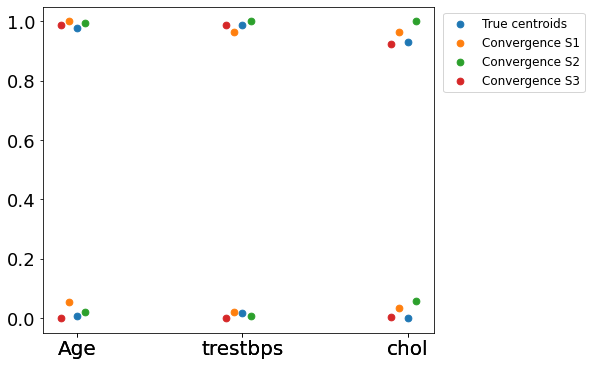
\includegraphics[scale=0.50]{figures/my_cluster_3.png}
\label{fig:cluster_free_3s} 
\end{figure}



%TC:endignore
\begin{table}[htbp]
\centering
 \setlength{\tabcolsep}{7pt} % Default value: 6pt 
 \renewcommand{\arraystretch}{1.35} % Default value: 1
  \captionsetup{justification=centering} 
\caption[Final Data points after convergence of clustering]{Final Data points after convergence; S1, S2 and S3 are the centroids obtained in each silo (S) after convergence; True centroids are the centroids of the true means of all silos (TC)}
\label{tab:datapoints}
\begin{tabular}{lccc}
\toprule
 & Age & trestbps & chol \\
\midrule
S1 & 46.3 , 61.1 & 121.1 , 148.9 & 218.9 , 300.8 \\
S2  & 45.8 , 61.0 & 120.7 , 149.9 & 220.9 , 304.0 \\
S3 & 45.5 , 61.0 & 120.5 , 149.6 & 216.1 , 297.4 \\
TC  & 45.6 , 60.8 & 121.0 , 149.6 & 215.8 , 297.9   \\

\bottomrule
\end{tabular}
\end{table}




%TC:ignore



\begin{figure}[H]
\centering
\captionsetup{justification=centering}
\caption[Clustering for 3 variables with 9 silos]{Clustering for 3 variables with 9 silos and true centroids of the true means (TC); 2 continuous and 1 categorical one hot encoded, The values were normalised for visualisation purposes with MinMax}\label{fig:cluster_mydata_9s} 
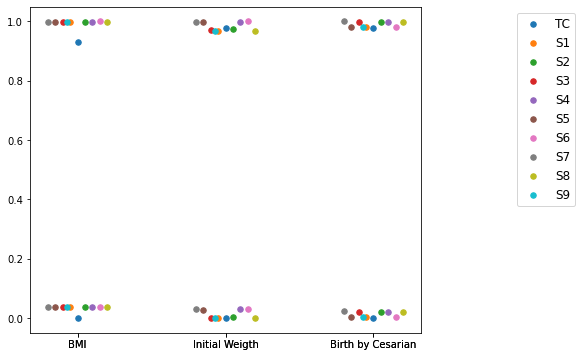
\includegraphics[scale=0.60]{figures/my_cluster_9.png}
\end{figure}
%TC:endignore

As before, the data is in table format in \ref{tab:datapoints_9}.

%%True Centroid & 24.9 , 25.3 & 66.6 , 65.6  & 0.24 , 0.29 \\

\begin{table}[htbp]
\centering
 \setlength{\tabcolsep}{7pt} % Default value: 6pt 
 \renewcommand{\arraystretch}{1.35} % Default value: 1
  \captionsetup{justification=centering} 
\caption{Final Data points after convergence and true centroids of the true means of each silo (TC)}
\label{tab:datapoints_9}
\begin{tabular}{lccc}
\toprule
 & \acs{bmi} & Initial Weight & Birth by Cesarian \\
\midrule
TC & 24.9 , 383.1 & 60.5 , 85.0  & 0 , 1 \\
S1 & 40.1 , 409.4 & 60.4 , 85.0 & 0.96 , -0.04 \\
S2 & 40.1 , 410.4 & 61.7 , 86.3 & 0.99 , -0.01 \\
S3 & 40.0 , 410.4 & 61.9 , 86.5 & 0.96 , -0.04 \\
S4 & 40.6 , 411.3 & 61.9 , 86.5 & 0.96 , -0.04 \\
S5 & 40.0 , 410.4 & 60.5 , 85.1 & 1.0 , 0.0 \\
S6 & 40.1 , 409.3 & 60.4 , 84.9 & 1.0 , 0.0 \\
S7 & 40.7 , 411.3 & 60.5 , 85.0 & 0.96 , -0.04 \\
S8 & 40.0 , 410.4 & 86.5 , 61.9 & 1.0 , 0.0 \\
S9 & 41.0 , 410.4 & 85.0 , 60.4 & 1.0 , 0.0 \\
\bottomrule
\end{tabular}
\end{table}




Then we experimented with categorical variables. Figure \ref{fig:cluster_3_cat} shows the convergence of the silos with proportion data and K-means with that and with K-modes.
\begin{figure}[ht]
\caption{Clustering for 3 variables with 3 silos - (A) categorical variables with  proportion with K-Means and (B)  Categorical with K-modes  }\label{fig:cluster_3_cat} 
  \subcaptionbox*{(A)}[.60\linewidth]{%
    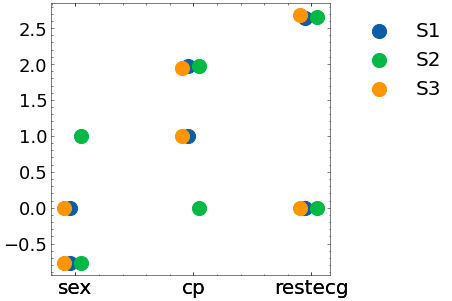
\includegraphics[width=\linewidth]{figures/my_cluster_3_cat.png}%
  }%
  \hfill
  \subcaptionbox*{(B)}[.44\linewidth]{%
    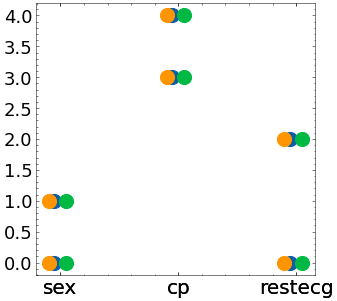
\includegraphics[width=\linewidth]{figures/my_cluster_3_cat_kmodes.png}%
  }
\end{figure}


\subsection{Discussion}
As per the discussion, there are a few issues to be addressed. First as per data preprocessing. In order to cluster be obtained, the null data must be filled out. There are a few strategies to do so. One option is to eliminate records/rows with empty cells or impute data. Either is a possibility, with pros and cons but the capability of having a dataset where no null records are present across several features may be difficult to find in the wild, especially since there are often optional and conditional fields in most Electronic Health Records (EHR). So imputation becomes more interesting, since it enables the usage of the whole dataset, even if biases are introduced.
Mixed types of datasets are also an issue to be aware of. In this case, not only imputation but also encoding a categorical variable is a vital step to take in the preprocessing phase. There are usually two main methods of data encoding, ordinal encoding and binary encoding. The first one keeps a unique column as the original data but maps every category to an increasing natural number. This creates an ordering in the data, often a misrepresentation of reality, not only due to this hierarchy but only because it assumes the differences between ranks of the hierarchy are always the same (1). The second is related to expanding the number of columns into the number of categories and creating 0s and 1s for the category. In machine-learning terms, binary seems more suited to be applied, but for benchmarking purposes, both are below par in terms of interpretability. For categorical data, we found out that K-modes seem to fulfil the requirements in a better way, providing better interpretability and reasoning about the results. However, it should be noted that we applied K-modes in a multivariate fashion and K-means in a univariate fashion.
Given that no percentage is provided, only the mode of the data, we believe it is still hard to get any real insight from the centroids. However, K-modes provides less information, since it only shows the top two categories. Which, for example. binary targets, provide little to no information. However, for larger categorical sets, the information provided could be better. Moreover, the number of centroids pretended could be more important as well. Agreeing on only 1 centroid would render the mode of the data provided by all silos, which could be more interesting.
As for continuous data, the use of real data was insightful, since BMI had a few very big outliers around 300 and 400, which rendered centroids around that data. Even if not all silos had examples of these outliers, the ones that do have, pass that into the remaining. One possible workaround would be an addition of an extra cluster in order to catch possible outliers.
However, this should be addressed in detail and assess how outliers could subvert the data from the silos and how to work around that.

% should be addressed more in focus since it was outside of the scope of this paper
As for the next steps, a few issues could be addressed in depth. Regarding imputation, it could be interesting to understand how imputation, and which methods are more suitable to use for real-world scenarios. If the imputation of variables with a high null percentage influence significantly a centroid formation.
Communication could be important as well. Which action is to be taken when a silo is "down" and does not send information to the remaining. Cluster information should be addressed as well. They need to be agreed upon beforehand in the scope of this paper. But if it could be selected by each silo? Would that be feasible or a convergence could be achieved?
Finally, there is the question if there is the possibility of having leaks of true means across iterations by adversarial learning. At present time, we cannot be sure that the values are totally private, but then again, nothing is.


% abordar na questao a vantagem da privacidade mas que é possivel haver leak dos valores por adervisal learning.

\subsection{Conclusion}
We believe that this work helps create the foundation for exchanging data across healthcare institutions without revealing the true data points. It could be useful for benchmarking and promoting a higher adoption rate.
Even though there are still issues to be addressed, we think that the path is full of possibilities.



